\documentclass[MATH-115-Notes.tex]{subfiles}

\begin{document}
\onecolumn
\chapter{Math 115 Past Finals}
\section{F17-MATH 115 Final Examination Part 1 (MC)}
\begin{enumerate}[itemsep=5mm]
    
    \item Evaluate the improper integral \[\int_{1}^{\infty}\frac{dx}{x^2}\]
    \begin{tasks}(4)
        \task 1/4  
        \task 1
        \task 2
        \task 4
        \task 1/2
        \task 3
        \task 1/3
        \task divergent
    \end{tasks}
    \paragraph*{Solution}
    \begin{gather*}
        \lim_{r \to \infty}\int_{1}^{r}\frac{dx}{x^2}\\
        \lim_{r \to \infty} \frac{-1}{x}\Big|_1^r\\
        \lim_{r \to \infty} \frac{-1}{r} - \frac{-1}{1}\\
        0 - (-1)\\
        = 1\\
        \text{The answer is b}
    \end{gather*}
    
    \item Evaluate the improper integral \[\int_{1}^{\infty}\frac{dx}{\sqrt{x}}\]
    \begin{tasks}(4)
        \task 1/4  
        \task 1
        \task 2
        \task 4
        \task 1/2
        \task 3
        \task 1/3
        \task divergent
    \end{tasks}
    \paragraph*{Solution}
    \begin{gather*}
        \lim_{r \to \infty}\int_{1}^{r}\frac{dx}{\sqrt{x}}\\
        \lim_{r \to \infty} 2\sqrt{x}\Big|_0^r\\
        \lim_{r \to \infty} 2\sqrt{r} - 2\sqrt{1}\\
        \infty - 2 \rightarrow \infty\\
        = \infty\\
        \text{The answer is h, it's diverges}
    \end{gather*}
    \item Evaluate the improper integral \[\int_{0}^{1}\frac{dx}{x^2}\]
    \begin{tasks}(4)
        \task 1/4  
        \task 1
        \task 2
        \task 4
        \task 1/2
        \task 3
        \task 1/3
        \task divergent
    \end{tasks}
    \paragraph*{Solution} 
    \begin{gather*}
        \lim_{r \to 0^+} \int_{r}^{1}\frac{dx}{x^2}\\
        \lim_{r \to 0^+} \frac{-1}{x}\Big|_r^1\\
        \lim_{r \to 0^+} \frac{-1}{1}-\frac{-1}{r}\\
        -1 - -\infty\\
        = \infty\\
        \text{The answer is h, it's divergent}
    \end{gather*} 
    
    \item Evaluate the improper integral \[\int_{0}^{1}\frac{dx}{\sqrt{x}}\]
    \begin{tasks}(4)
        \task 1/4  
        \task 1
        \task 2
        \task 4
        \task 1/2
        \task 3
        \task 1/3
        \task divergent
    \end{tasks}
    \paragraph*{Solution}
    \begin{gather*}
        \lim_{r \to 0^+}\int_{r}^{1}\frac{dx}{\sqrt{x}}\\
        \lim_{r \to 0^+} 2\sqrt{x}\Big|_r^1\\
        \lim_{r \to 0^+} 2\sqrt{1} - 2\sqrt{r}\\
        2 - 0 \\ 
        = 2\\
        \text{The answer is c}
    \end{gather*}
    
    \item Evaluate the improper integral \[\int_{0}^{1}\frac{\ln x}{x}\ dx\]
    \begin{tasks}(4)
        \task 1/2   
        \task 1
        \task 2
        \task \(\frac{1}{4}\ln 2\)
        \task \(\frac{1}{2}\ln 2\)
        \task 3 
        \task 1/2
        \task divergent
    \end{tasks}
    \paragraph*{Solution}
    \begin{gather*}
        \lim_{r \to 0^+}\int_{r}^{1}\frac{\ln x}{x}dx\\ 
        \text{Let u} = \ln x\\
        \text{du} = \frac{1}{x}dx\\
        \lim_{r \to 0^+} \int_{r}^{1}u\ du\\
        \lim_{r \to 0^+} \frac{u^2}{2}\Big|_r^1\\
        \lim_{r \to 0^+} \frac{\ln^2 1}{2} - \frac{\ln^2 r}{2}\\
        \frac{0}{2}-\frac{\infty}{2}\\
        = -\infty\\
        \text{The answer is h, its divergent}
    \end{gather*}
    
    \item The value of the integral \[\int_{0}^{\pi}\sin(2x)\cos(x)\ dx\] is:
    \begin{tasks}(4)
        \task \(1/2\)
        \task \(\pi/4\)
        \task \(1\)
        \task \(3\pi/4\)
        \task \(4/3\)
        \task \(2/3\)
        \task \(\pi/2\)
        \task \(0\)
    \end{tasks}
    \paragraph*{Solution}
    \begin{gather*}
        \int_{0}^{\pi}\sin(2x)\cos(x)dx\\
        \int_{0}^{\pi}2\sin(x)\cos(x)\cos(x)dx\\
        2\int_{0}^{\pi}\sin(x)\cos^2(x)dx\\
        \text{Let } u = \cos(x)\\
        \text{Then } du = -\sin(x)\\
        \text{I changed the domain from radians to real by inputing the original values into cos(x) to get 1 and -1.}\\
        -2\int_{1}^{-1}u^2du\\
        2\int_{-1}^{1}u^2du\\
        \frac{2}{3}u^3\Big|_{-1}^1\\
        \frac{2}{3}-\frac{-2}{3}\\
        = \frac{4}{3}\\
        \text{The answer is e}
    \end{gather*}
    \newpage

    \item The value of the integral \[\int_{0}^{\pi/4}\tan(x)\sec^2(x)\ dx\] is:
    \begin{tasks}(4)
        \task \(1/2\)
        \task \(\pi/4\)
        \task \(1\)
        \task \(3\pi/4\)
        \task \(\pi/2\)
        \task \(1/4\)
        \task \(3/4\)
        \task \(0\)
    \end{tasks}
    \paragraph*{Solution}
    \begin{gather*}
        \int_{0}^{\pi/4}\frac{\sin(x)}{\cos(x)}\frac{1}{\cos^2(x)}dx\\
        \int_{0}^{\pi/4}\frac{\sin(x)}{\cos^3(x)}dx\\
        \text{Let } u = \cos(x)\\
        \text{Then } du = -\sin(x)dx\\
        \text{I changed the domain from radians to real by inputing the original values into cos(x) to get 1 and $1/\sqrt{2}$}\\
        -\int_{1}^{1/\sqrt{2}}\frac{du}{u^3}du\\
        \int_{1/\sqrt{2}}^{1}\frac{du}{u^3}du\\
        -\frac{du}{2u^2}\Big|_{1/\sqrt{2}}^1\\
        -\frac{1}{2}-\frac{-1}{2\left(\frac{1}{\sqrt{2}}\right)^2}\\
        -\frac{1}{2}-\frac{-1}{\cancel{2}\frac{1}{\cancel{2}}}\\
        -\frac{1}{2}-\frac{-1}{1}\\
        = \frac{1}{2}\\
        \text{The answer is a.}
    \end{gather*}
    
    \item The slope to the tangent of the curve $x = \sin(t),\ y = \cos(t)$ when $t = \pi/3$ is:
    \begin{tasks}(4)
        \task \(-1/\sqrt{3}\)
        \task \(1/\sqrt{2}\)
        \task \(1/\sqrt{3}\)
        \task \(1\)
        \task \(-1\)
        \task \(-1\sqrt{3}\)
        \task \(\sqrt{3}\)
        \task \(-1/\sqrt{2}\)
    \end{tasks}
    \paragraph*{Solution}
    \begin{gather*}
        \text{The slope equation for a parametric curve is } m = \frac{dy}{dx}\\
        m(t) = \frac{\cos'(t)}{\sin'(t)}\\
        m(t) = \frac{-\sin(t)}{\cos(t)}\\
        m(\pi/3) = \frac{-\sin(\pi/3)}{\cos(\pi/3)}\\
        m = \frac{-\frac{\sqrt{3}}{2}}{\frac{1}{2}}\\
        m = -\frac{\sqrt{3}}{\cancel{2}} \frac{\cancel{2}}{1}\\
        m = -\sqrt{3}\\
        \text{The answer is g.}
    \end{gather*}


    \item The curve $x = t^2 - t,\ y = t^2 + t$ has a vertical tangent for $t$ equal to:
    \begin{tasks}(4)
        \task \(-1/3\)
        \task \(1/2\)
        \task \(-2\)
        \task \(1\)
        \task \(-1/2\)
        \task \(-3\)
        \task \(-1\)
        \task \(2\)
    \end{tasks}
    \paragraph*{Solution}
    \begin{gather*}
        \text{The slope equation for a parametric curve is } m = \frac{dy}{dx}\\
        m(t) = \frac{2t + 1}{2t - 1}\\
        \text{We want to find $t$ where the slope is vertical or $m = \infty$.}\\
        \frac{2t + 1}{2t - 1 \Rightarrow 0} \Rightarrow \pm\infty\\
        2t = 1\\
        t = \frac{1}{2}\\
        \text{Verifying}\\
        \frac{2\left( \frac{1}{2} \right) + 1}{2\left( \frac{1}{2} \right) - 1}\\
        \frac{\cancel{2}\left( \frac{1}{\cancel{2}} \right) + 1}{\cancel{2}\left( \frac{1}{\cancel{2}} \right) - 1}\\
        \frac{1 + 1}{1 - 1}\\
        \frac{2}{0} \Rightarrow \pm\infty\\
        \text{We now know that when $t = \frac{1}{2}$ the slope is vertical}\\
        \text{The answer is b.}
    \end{gather*}
    \newpage
    \item The slope to the tangent of the curve $x = t+ t^2,\ y = t + e^t$ at the point (0,1) is:
    \begin{tasks}(4)
        \task \(-3\)
        \task \(-2\)
        \task \(-1\)
        \task \(0\)
        \task \(1\)
        \task \(2\)
        \task \(3\)
        \task \(4\)
    \end{tasks}
    \paragraph*{Solution}
    \begin{gather*}
        \text{First we need to find t.}\\
        0 = t + t^2\\
        t = 0\\
        \text{The slope equation for a parametric curve is } m = \frac{dy}{dx}\\
        m(t) = \frac{1 + e^t}{1 + 2t}\\
        m(0) = \frac{1+e^0}{1+2(0)}\\
        m(0) = \frac{1 + 1}{1 + 0}\\
        m(0) = \frac{2}{1}\\
        m = 2\\
        \text{The answer is f.}
    \end{gather*}
\end{enumerate}
\newpage
\section{F17-MATH 115 Final Examination Part 2 (Long Answer)}
\begin{enumerate}
    \item Evaluate the following integral
    \begin{enumerate}
        \item \[\int_{}^{}\frac{\sqrt{x}}{6+x}dx\]
        \paragraph{Solution}~\\
        {\centering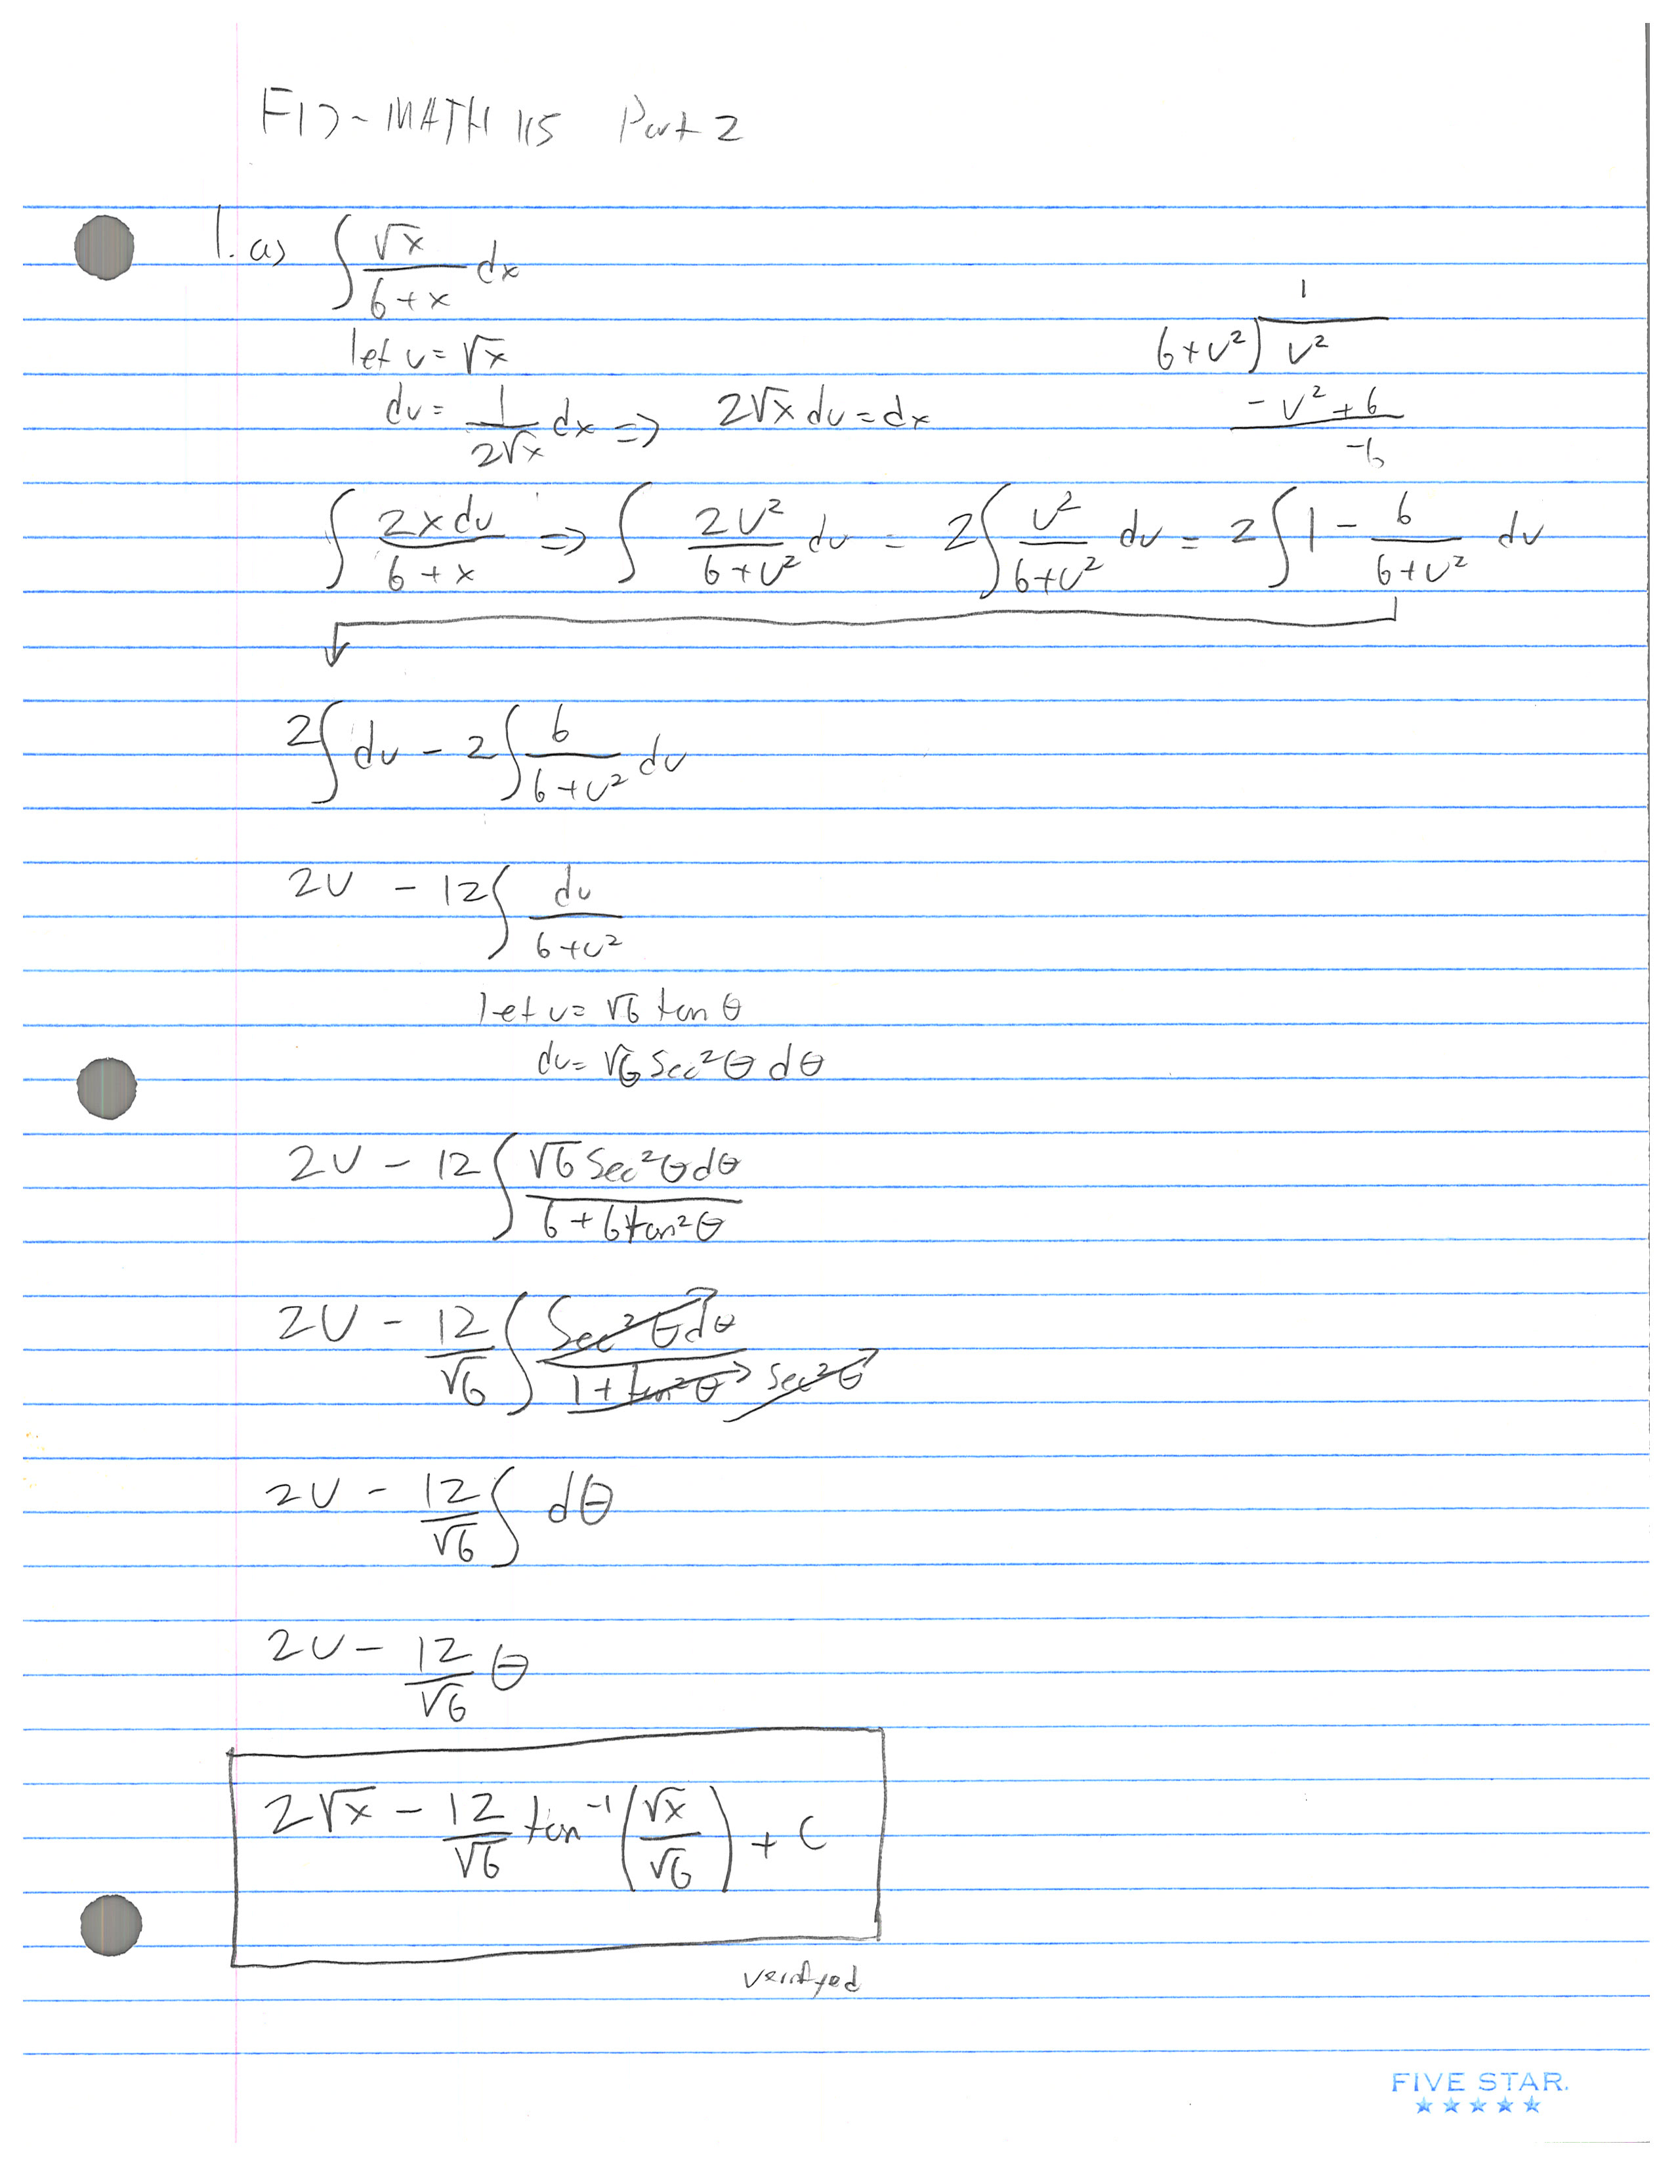
\includegraphics[trim={0 0 0 0},clip,scale=0.45]{./figures/math-final-work001.jpg}\\}
        \newpage
        \item \[\int_{}^{}\frac{x^3 + 2x}{\sqrt{x^2 - 1}}dx\]
        \paragraph{Solution}~\\
        {\centering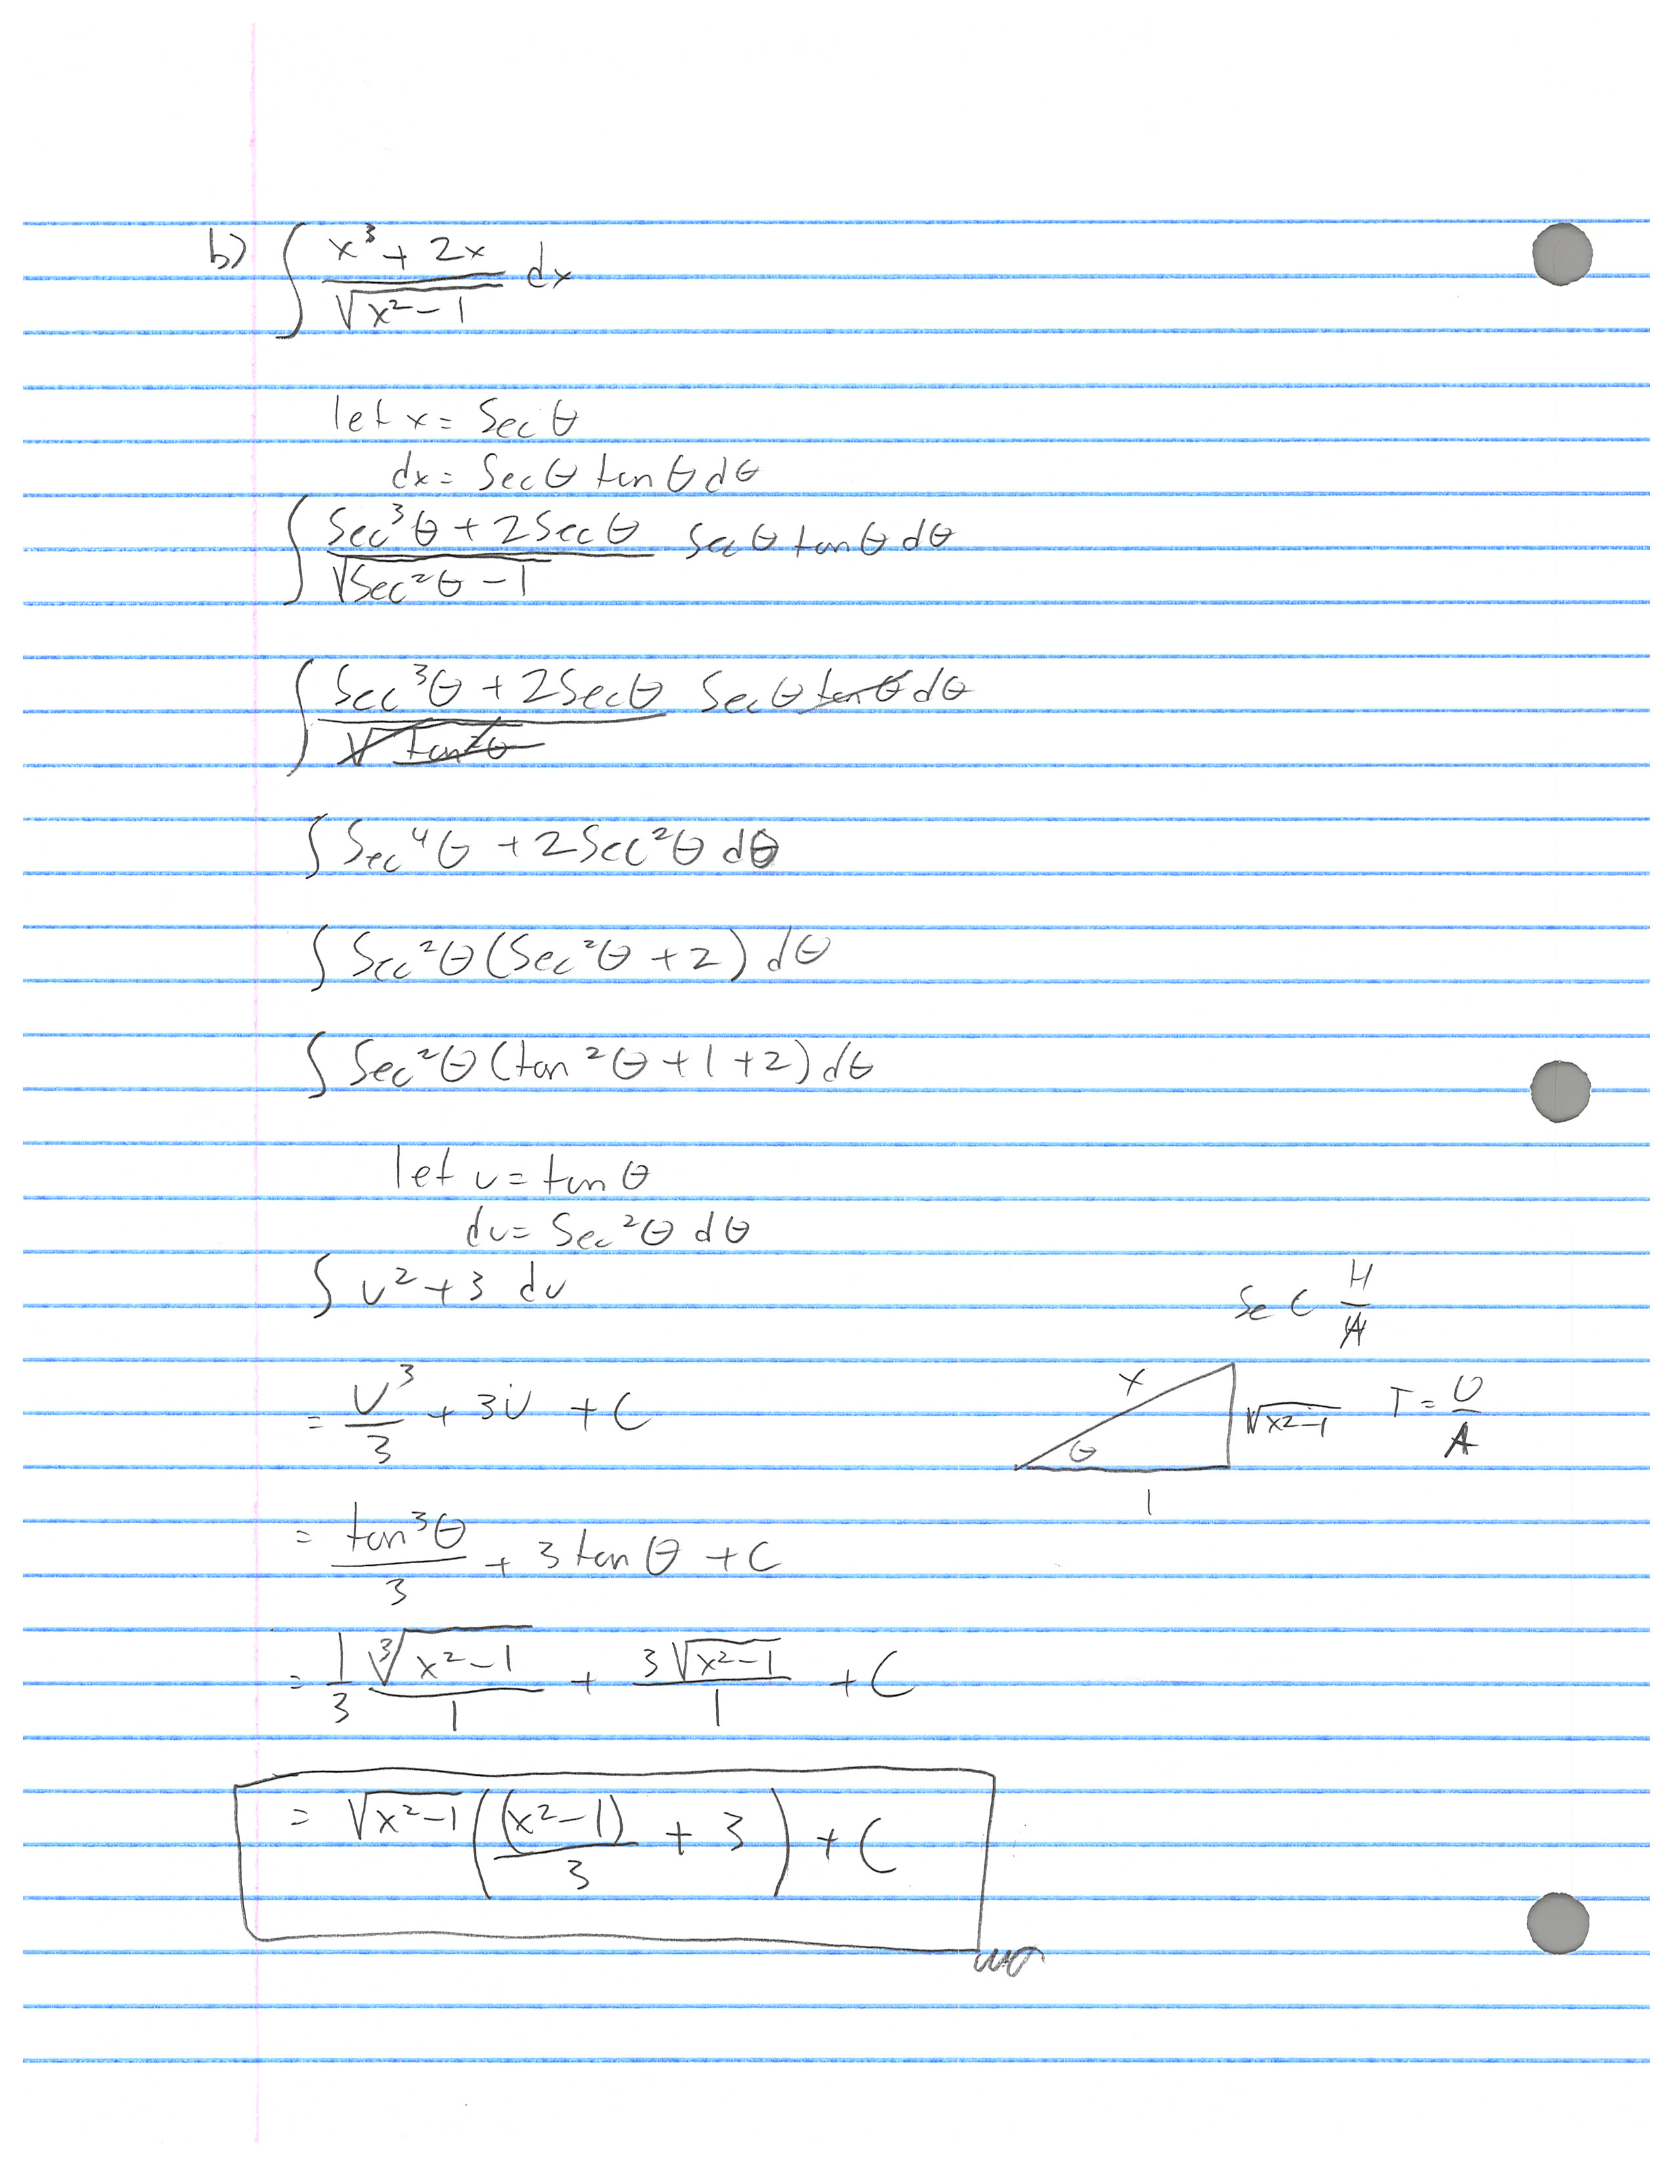
\includegraphics[trim={0 3cm 0 0},clip,scale=0.4]{./figures/math-final-work002.jpg}\\}
    \end{enumerate}
    
    \item Evaluate the following integrals:
    \begin{enumerate}
        \item \[\int_{}^{}\cos(\ln x)dx\]
        \paragraph{Solution}~\\
        {\centering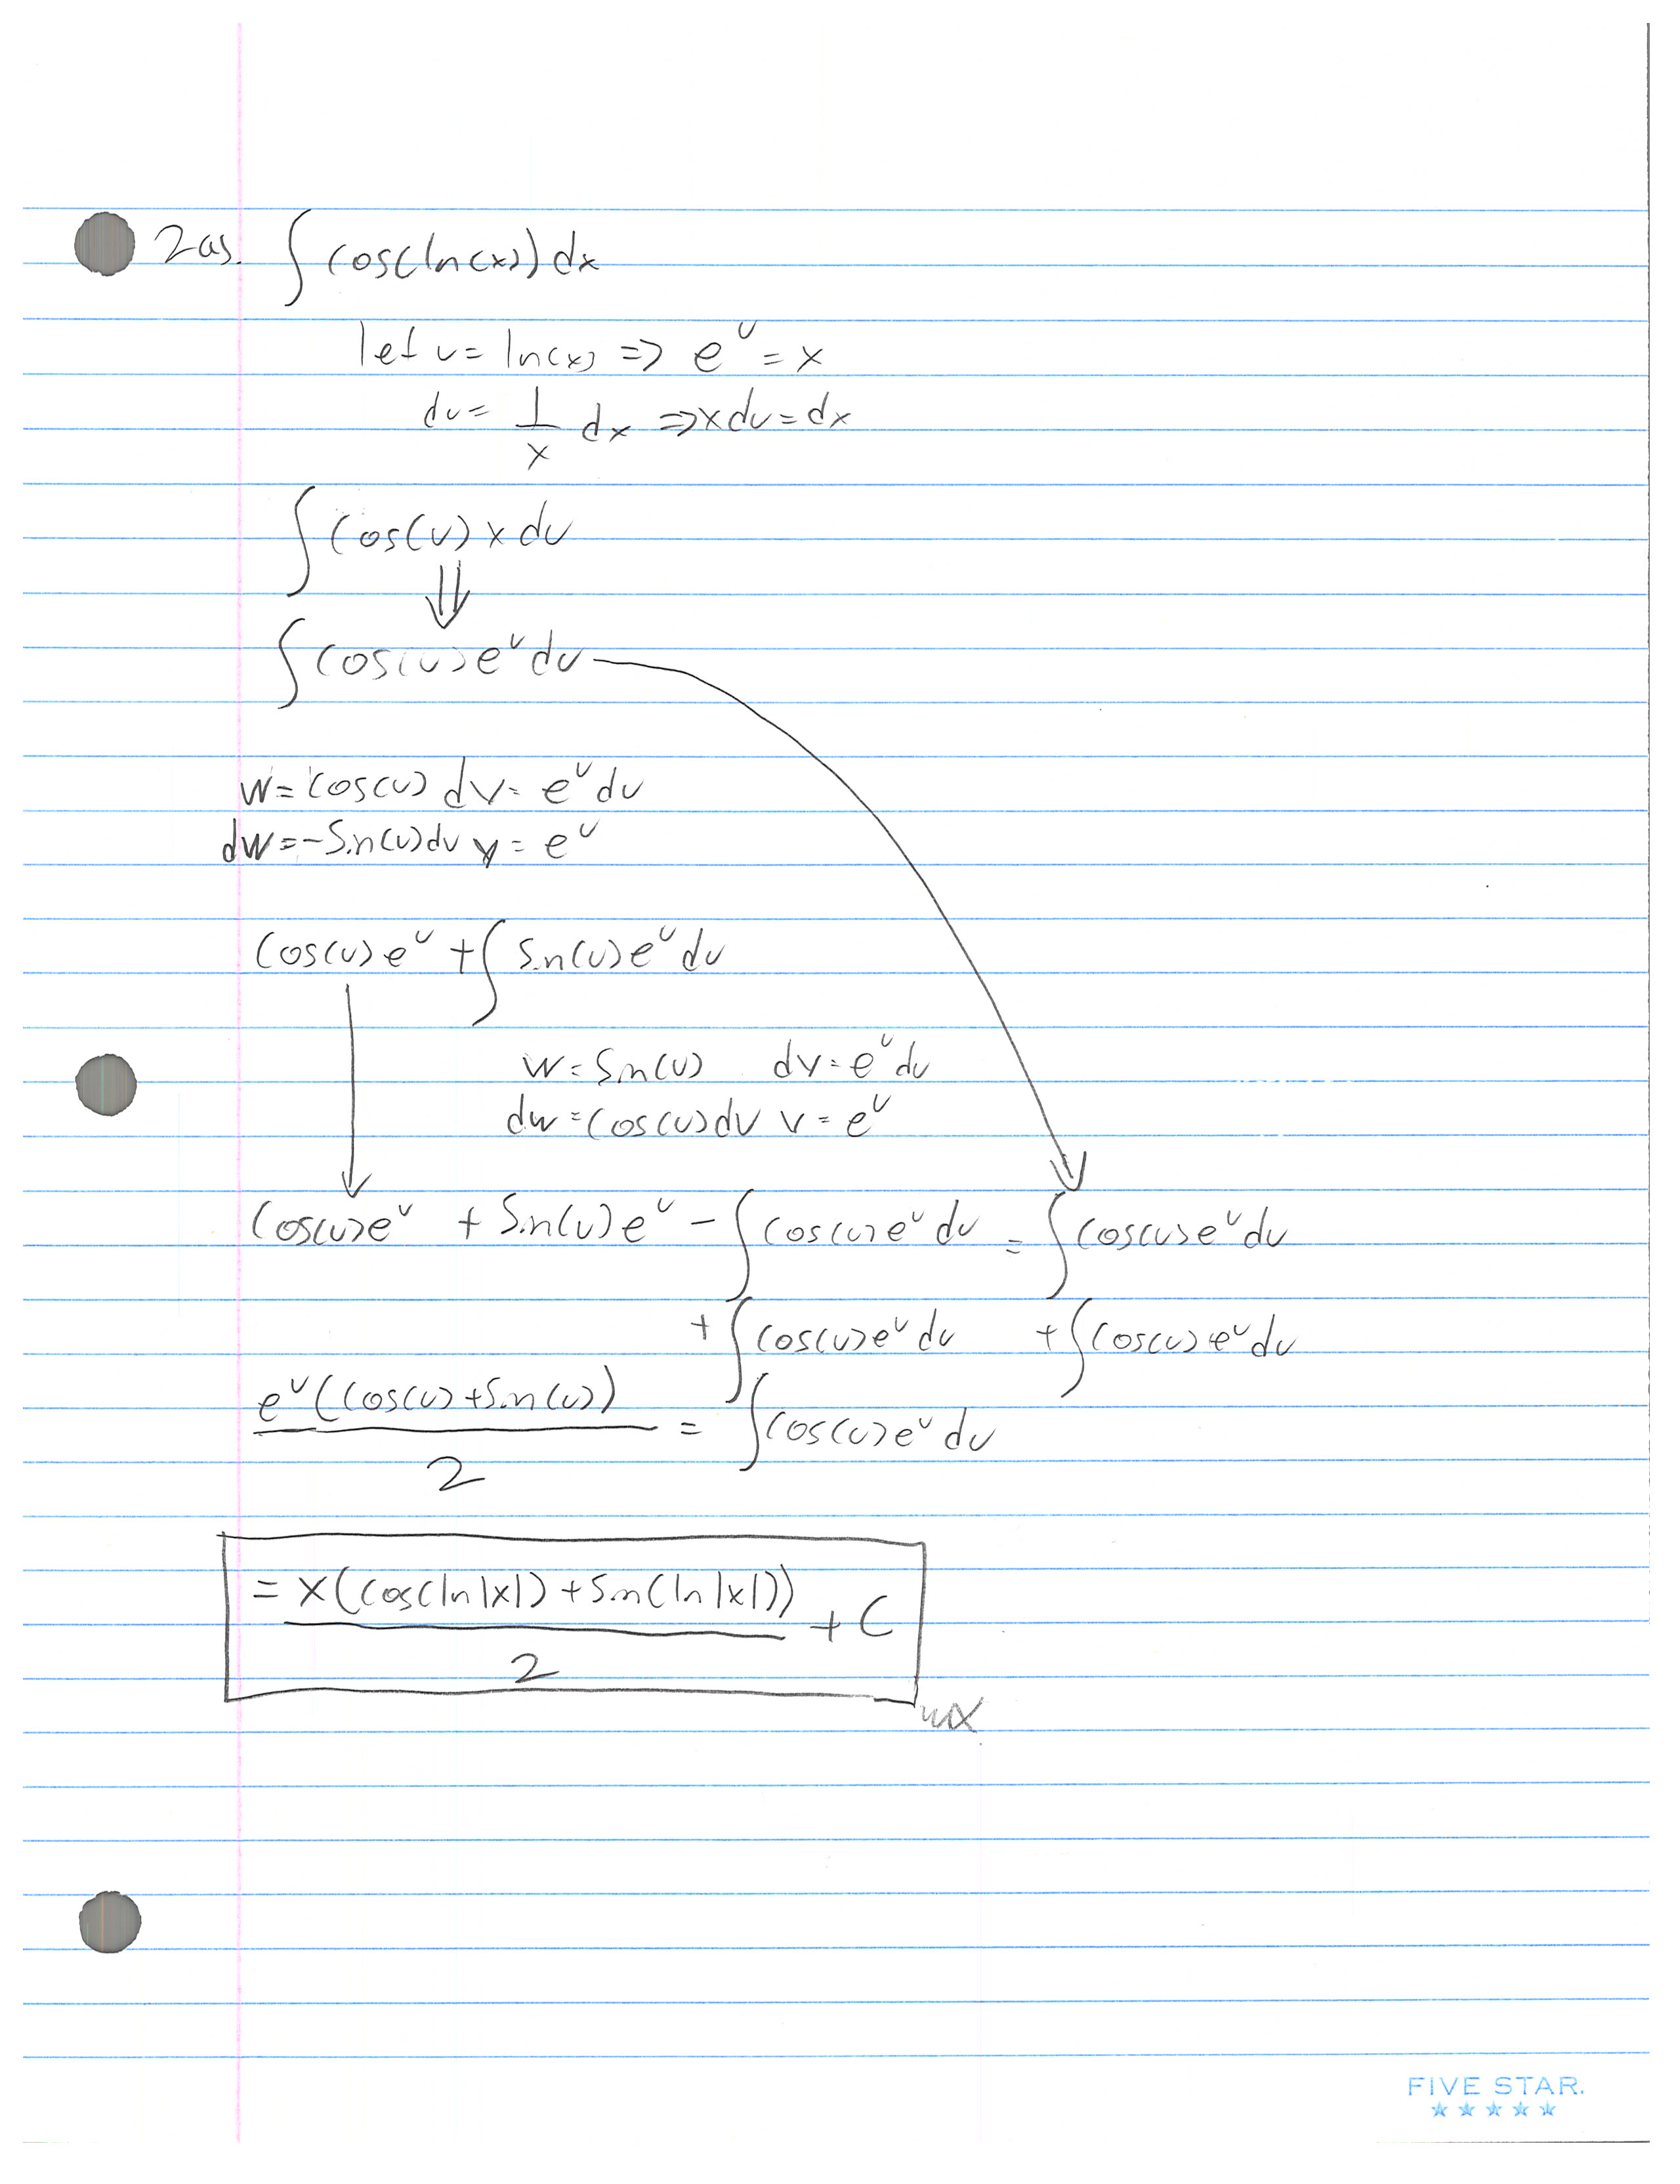
\includegraphics[trim={0 5cm 0 0},clip,scale=0.4]{./figures/math-final-work003.jpg}\\}
        \newpage
        \item \[\int_{}^{}\frac{x}{x^2+x-6}dx\]
        \paragraph{Solution}~\\
        {\centering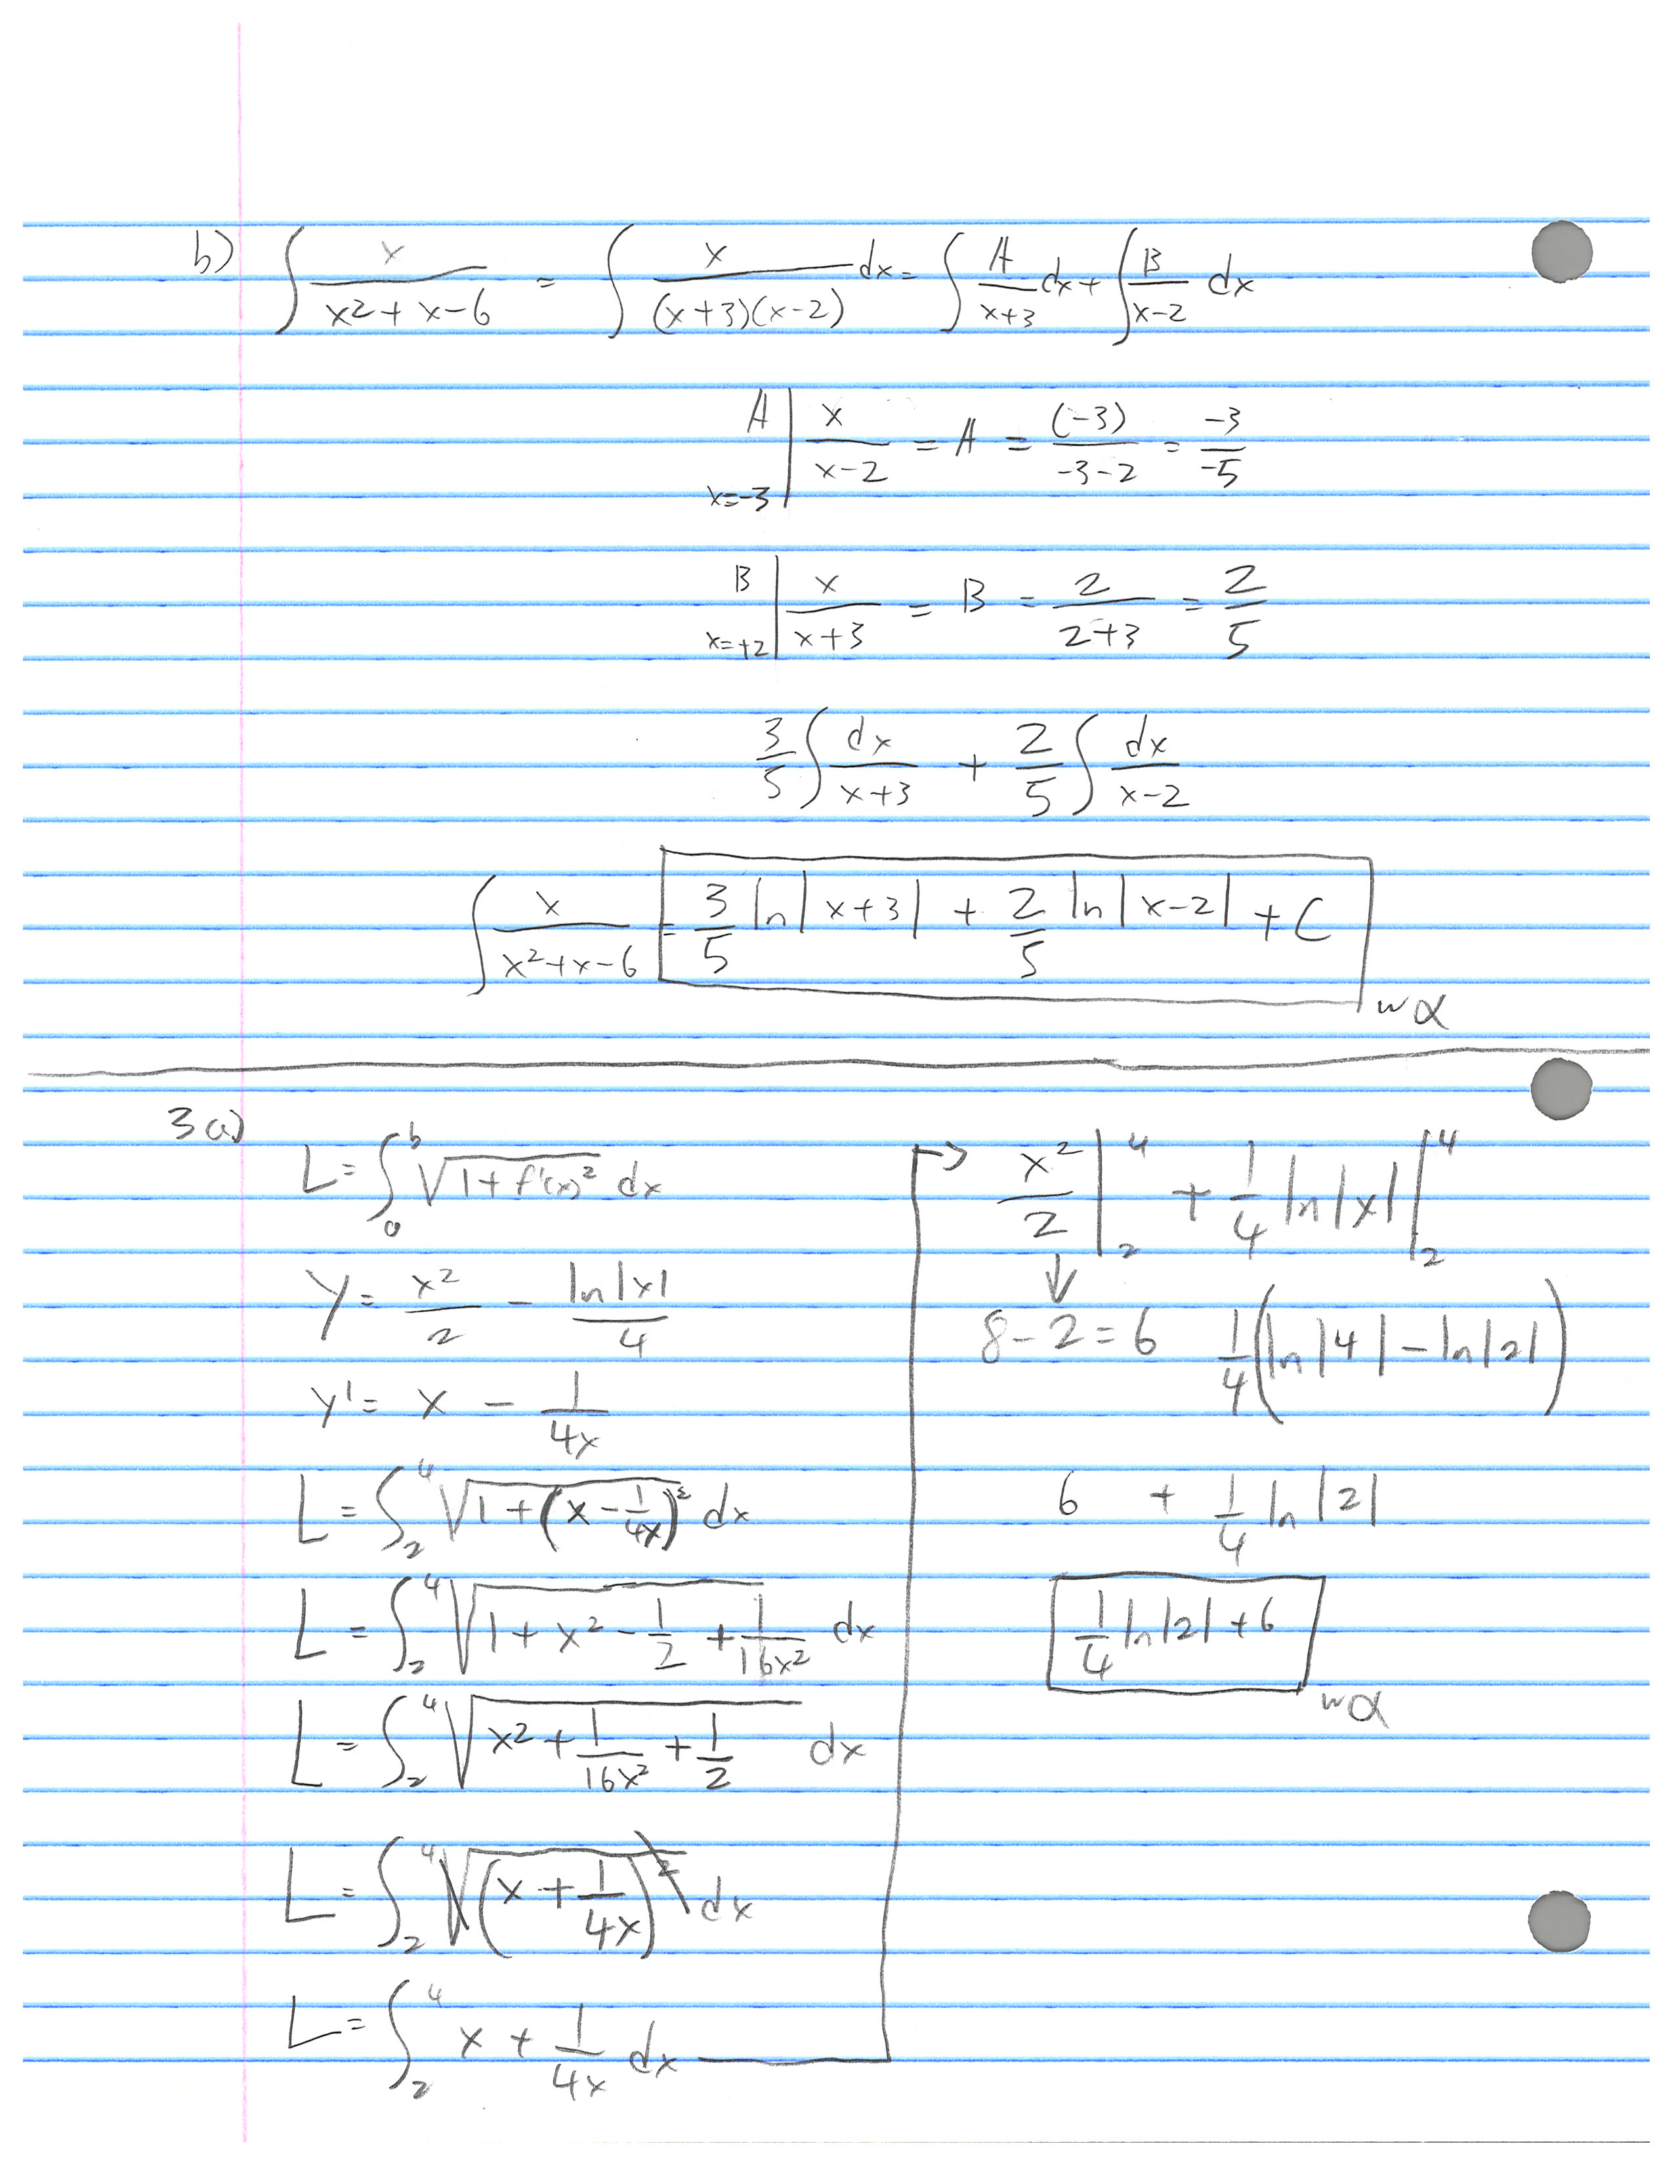
\includegraphics[trim={0 15cm 0 0},clip,scale=0.425]{./figures/math-final-work004.jpg}\\}
    \end{enumerate}
    
    \item\ \begin{enumerate}
        \item Find the arc length of the curve \[y = \frac{x^2}{2}-\frac{\ln x}{4},\ \text{for}\ 2 \leq x \leq4\]
        \paragraph{Solution}~\\
        {\centering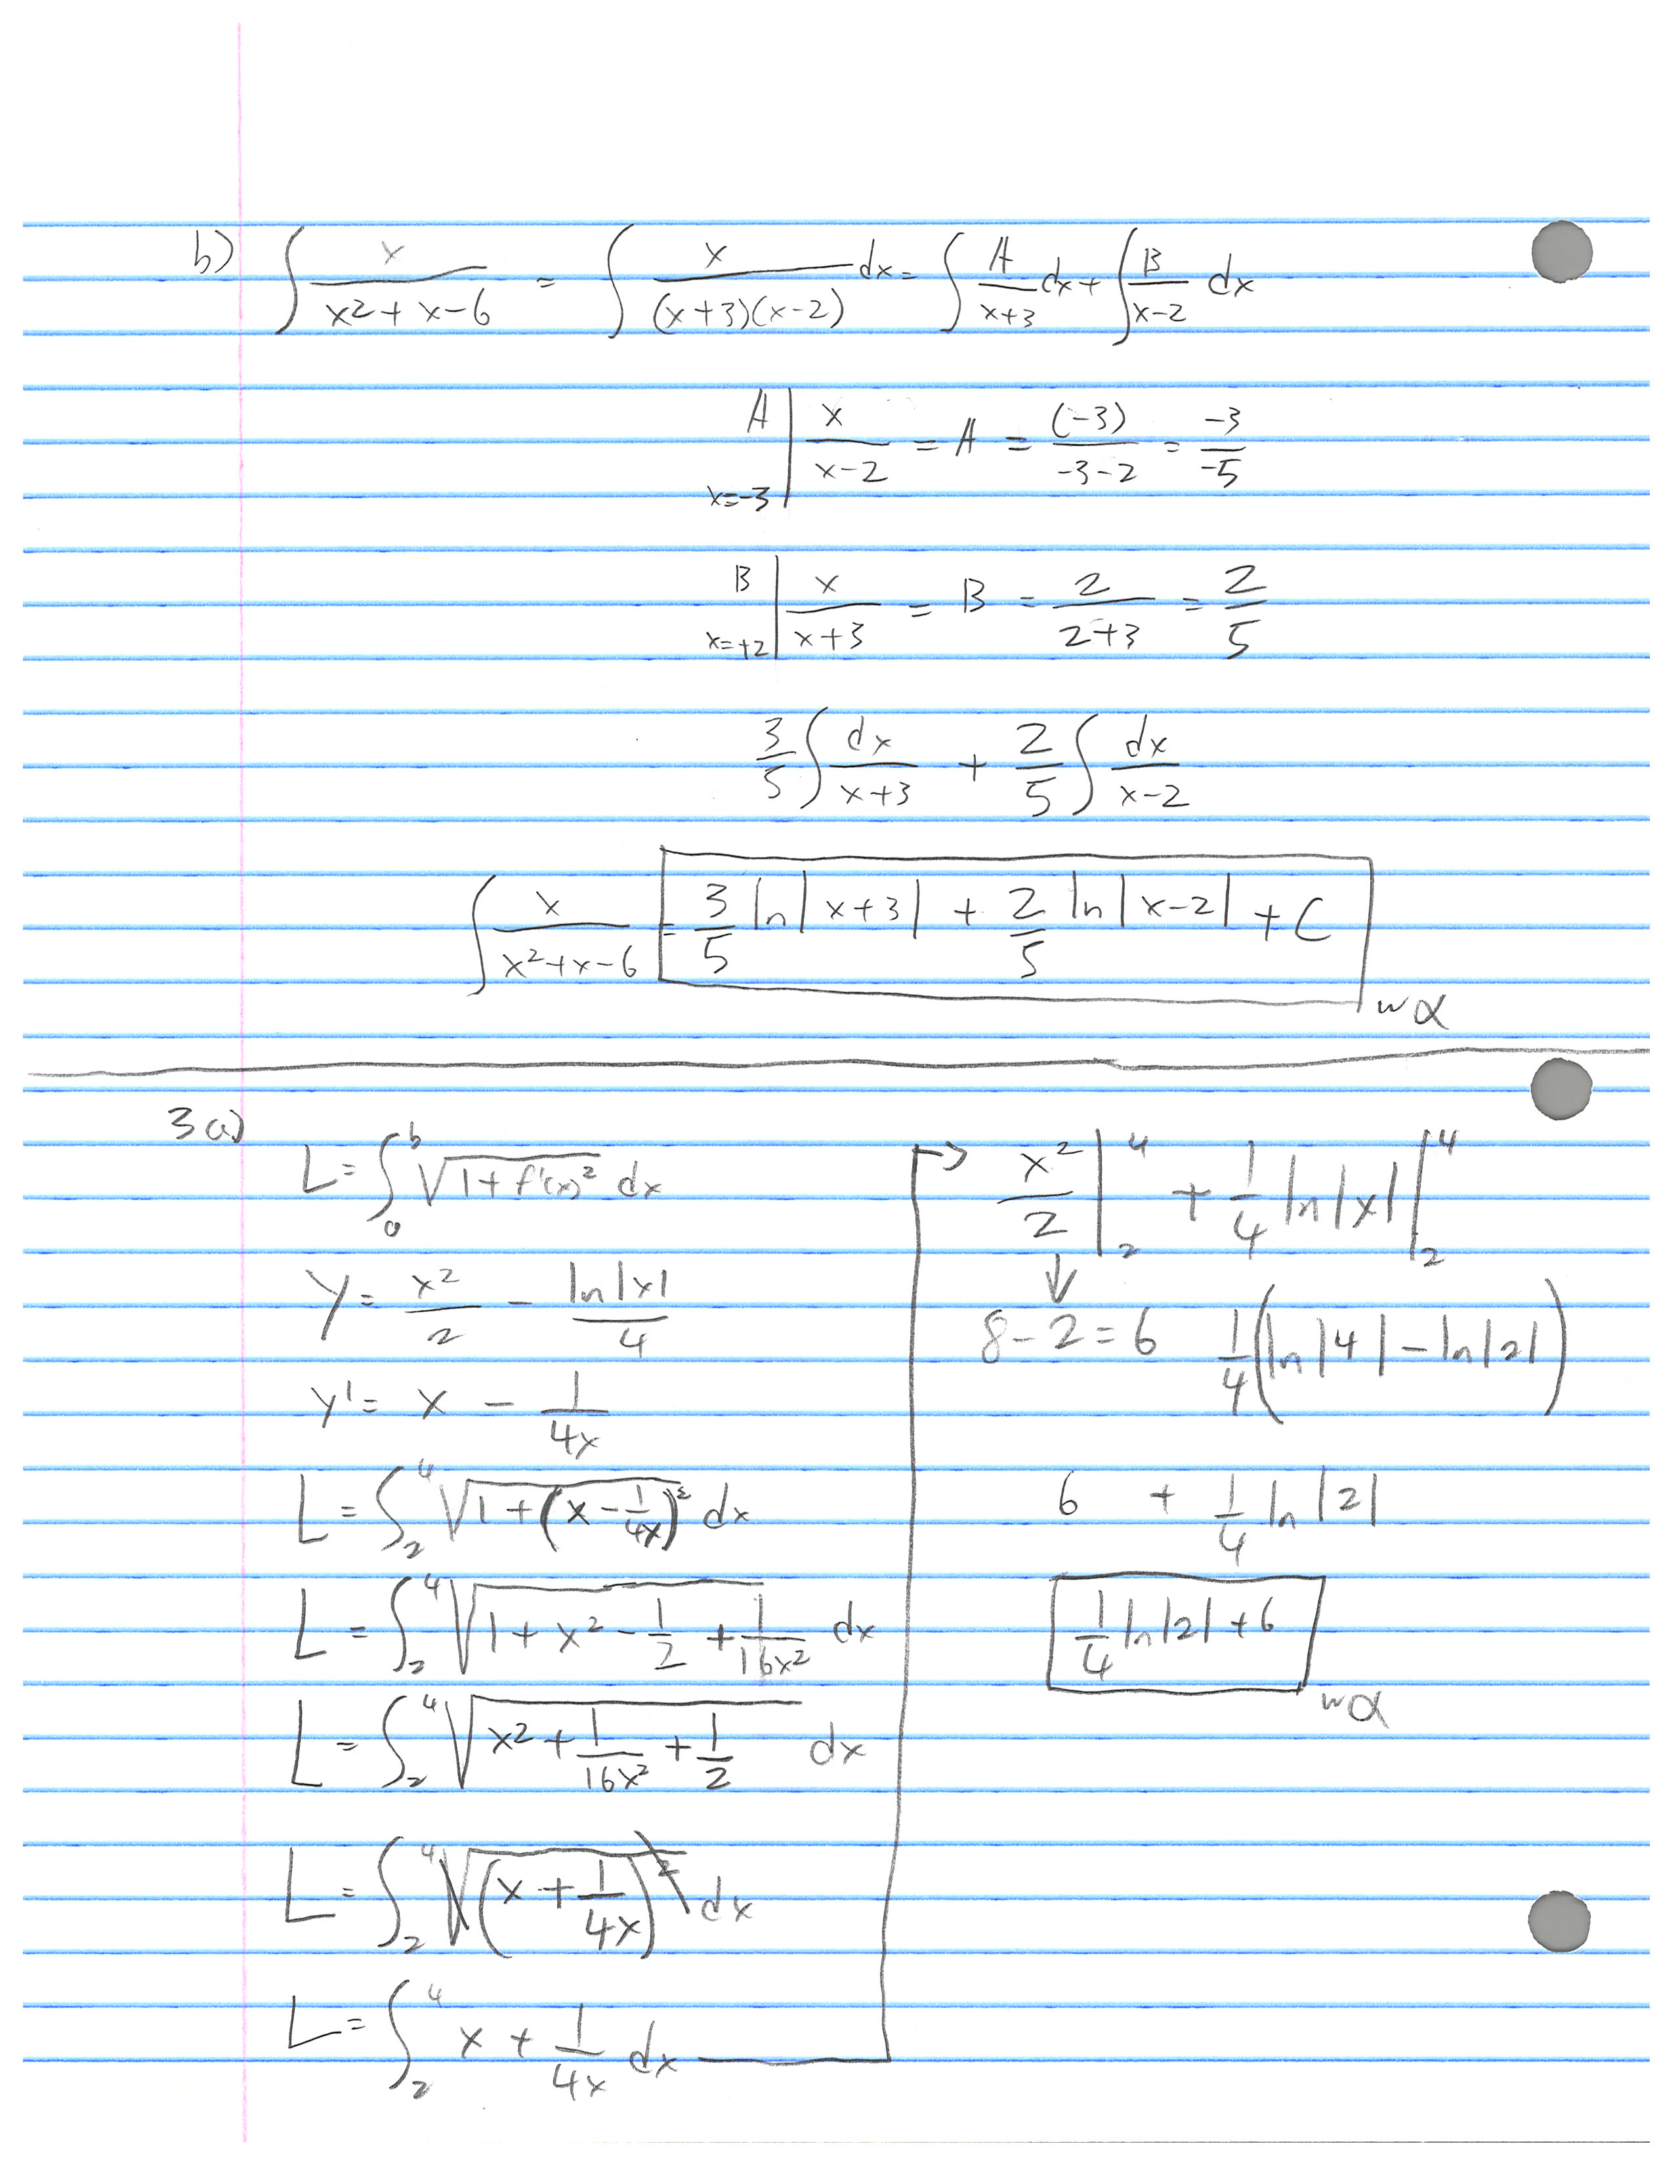
\includegraphics[trim={0 0 0 14cm},clip,scale=0.425]{./figures/math-final-work004.jpg}\\}
        \item Find the area of the surface generated by revolving the curve \(y = x^\frac{1}{3},\ \text{from}\ x = 0,\ \text{to}\ x = 1\) about the y-axis.
        \paragraph{Solution}~\\
        {\centering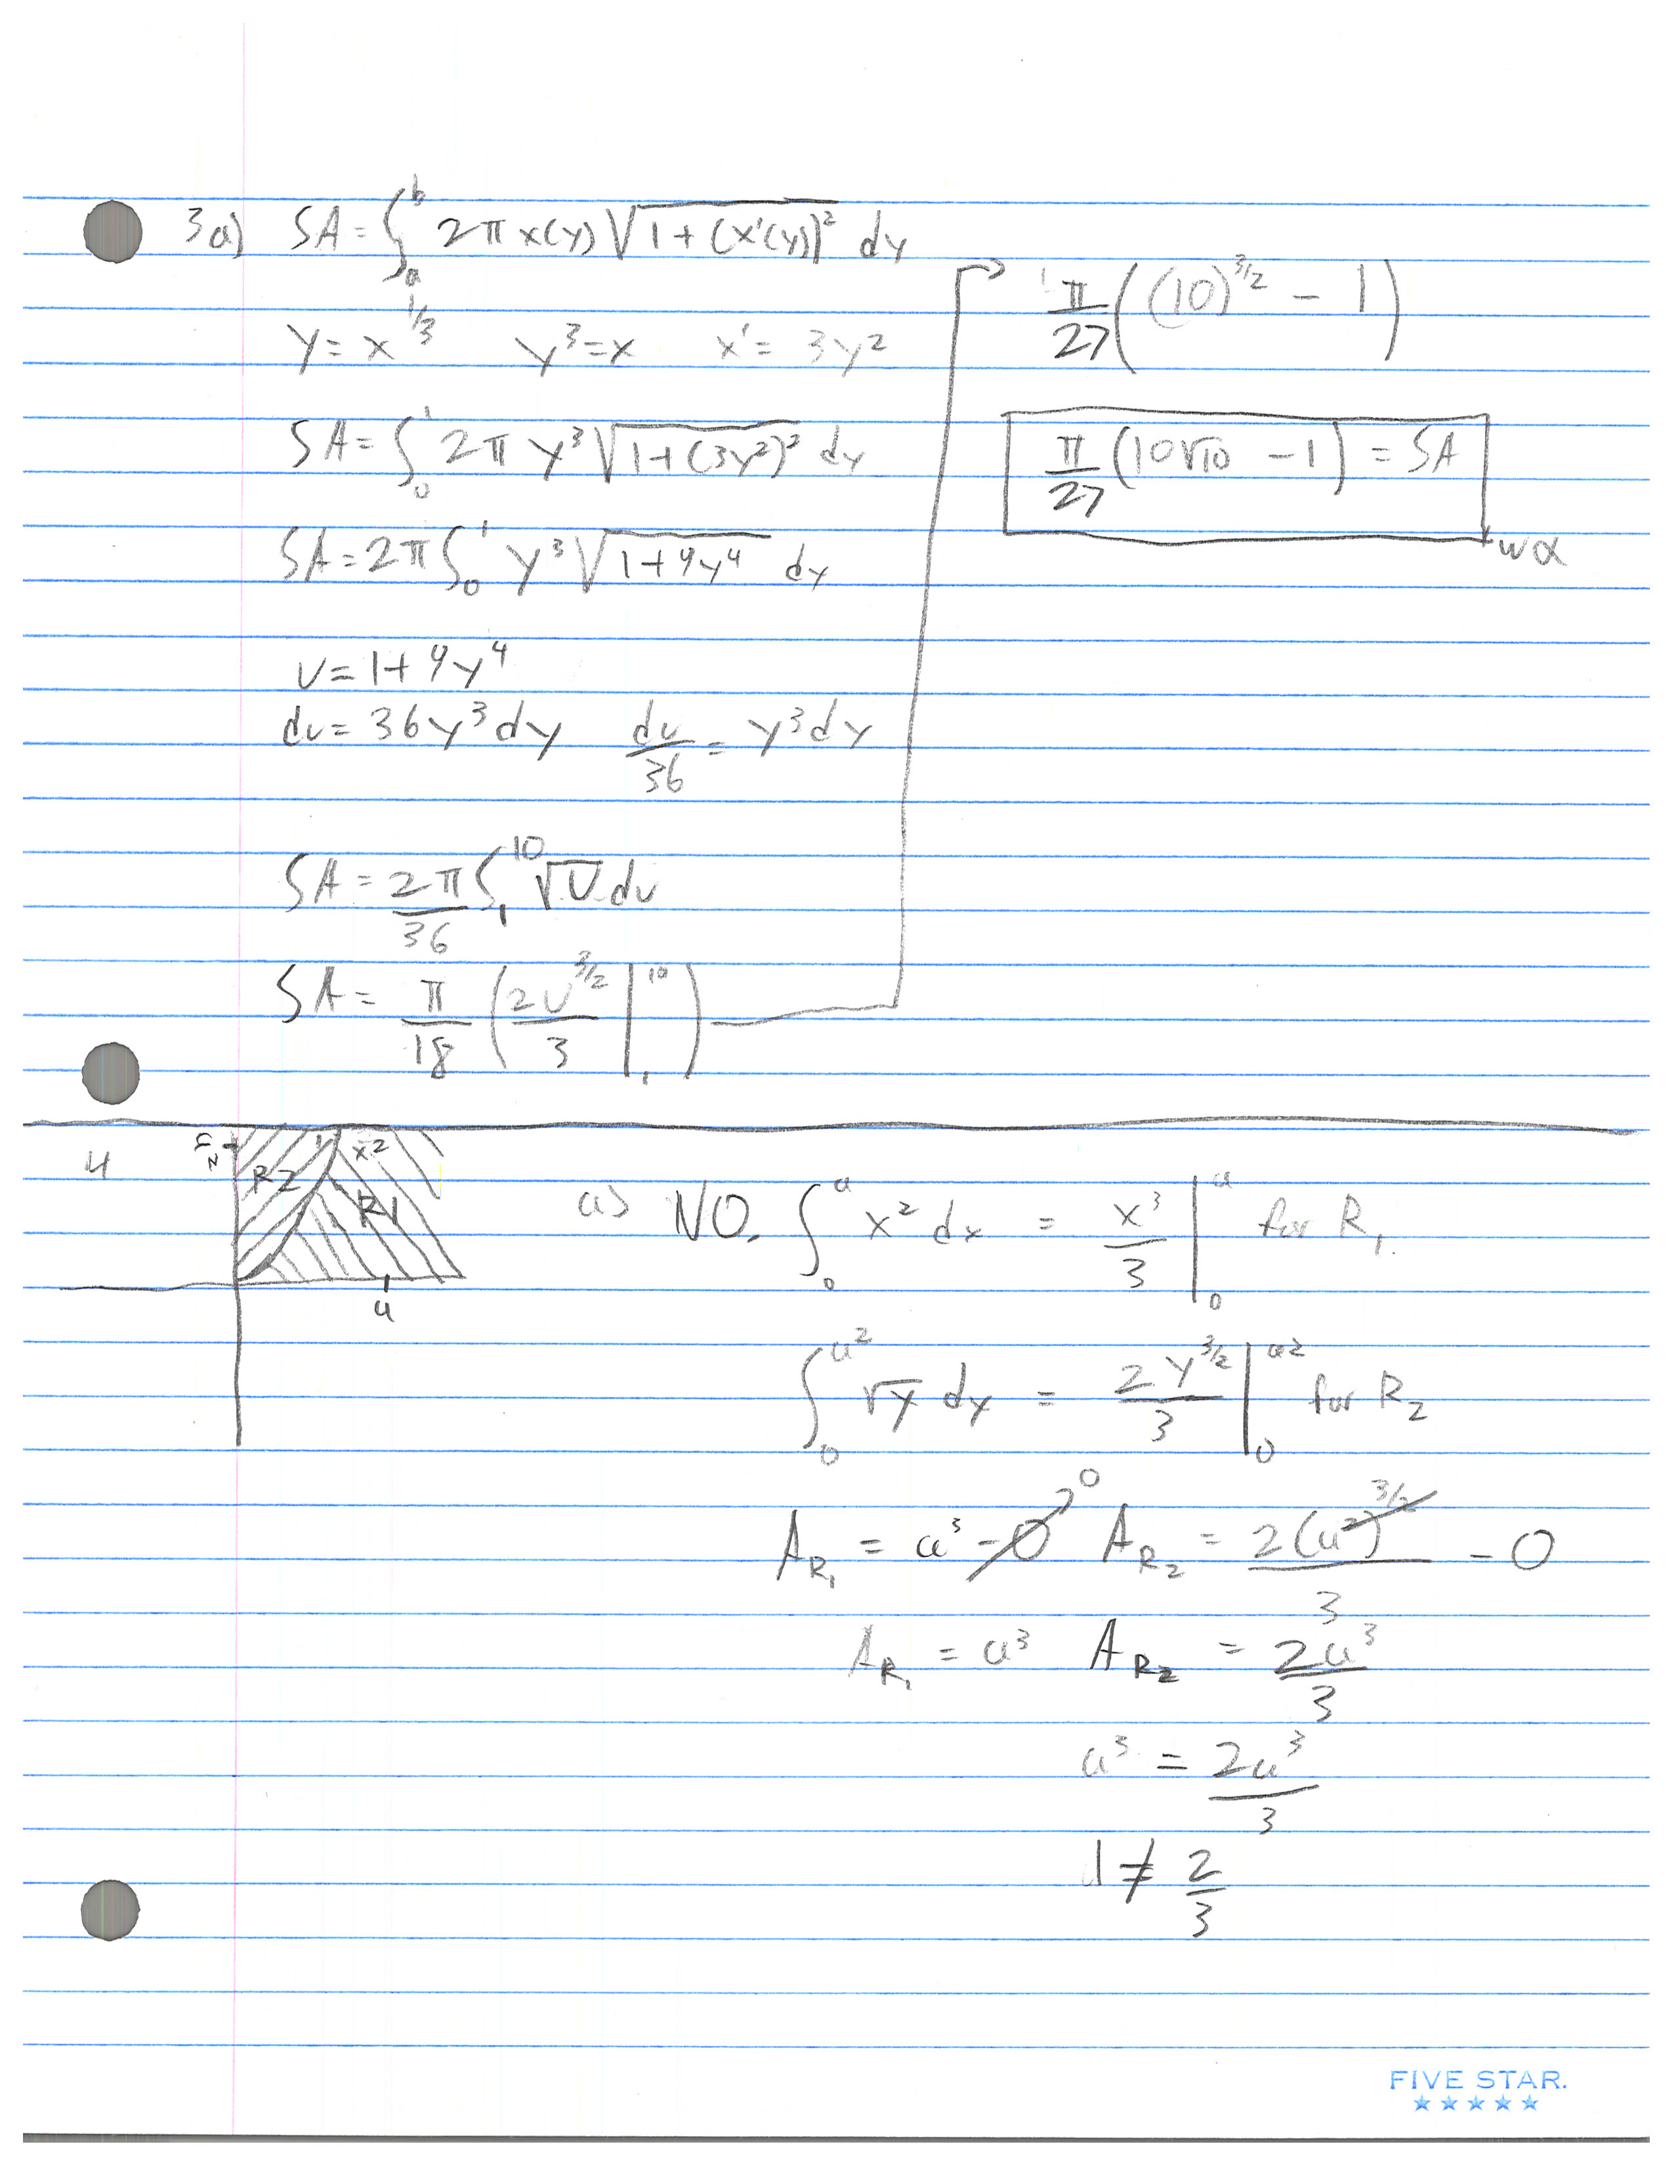
\includegraphics[trim={0 14cm 0 0},clip,scale=0.425]{./figures/math-final-work005.jpg}\\}
        I changed the domain during the substitution of $u$. 
    \end{enumerate}
    
    \item Let $\mathcal{R}_1$ be the region bounded by \(y = x^2,\ y = 0\) and \(x = a\) where \(a > 0\). Let \(\mathcal{R}_2\) be the region bounded by \(y = x^2,\ x = 0\) and \(y = a^2\).
    \begin{enumerate}
        \item Is there a positive value of $a$ such that $\mathcal{R}_1$ and $\mathcal{R}_2$ have the same area? Justify your answer.
        \paragraph{Solution}
        No as shown below:
        \begin{gather*}
            A_{\mathcal{R}_1}\int_{0}^{a} x^2 dx = \frac{x^3}{3}\Big|_0^a\\
            A_{\mathcal{R}_2}\int_{0}^{a^2} \sqrt{y}\ dy = \frac{2y^{3/2}}{3}\Big|_0^{a^2}\\
            A_{\mathcal{R}_1} = a^3,\qquad A_{\mathcal{R}_2} = \frac{2a^3}{3} \\
            a^3 \neq \frac{2a^3}{3} 
        \end{gather*}

        \item Is there a positive value of $a$ such that $\mathcal{R}_1$ sweeps out the same volume when rotated about the x-axis as it does when rotated about the y-axis? Justify your answer.
        \paragraph{Solution}~\\
        {\centering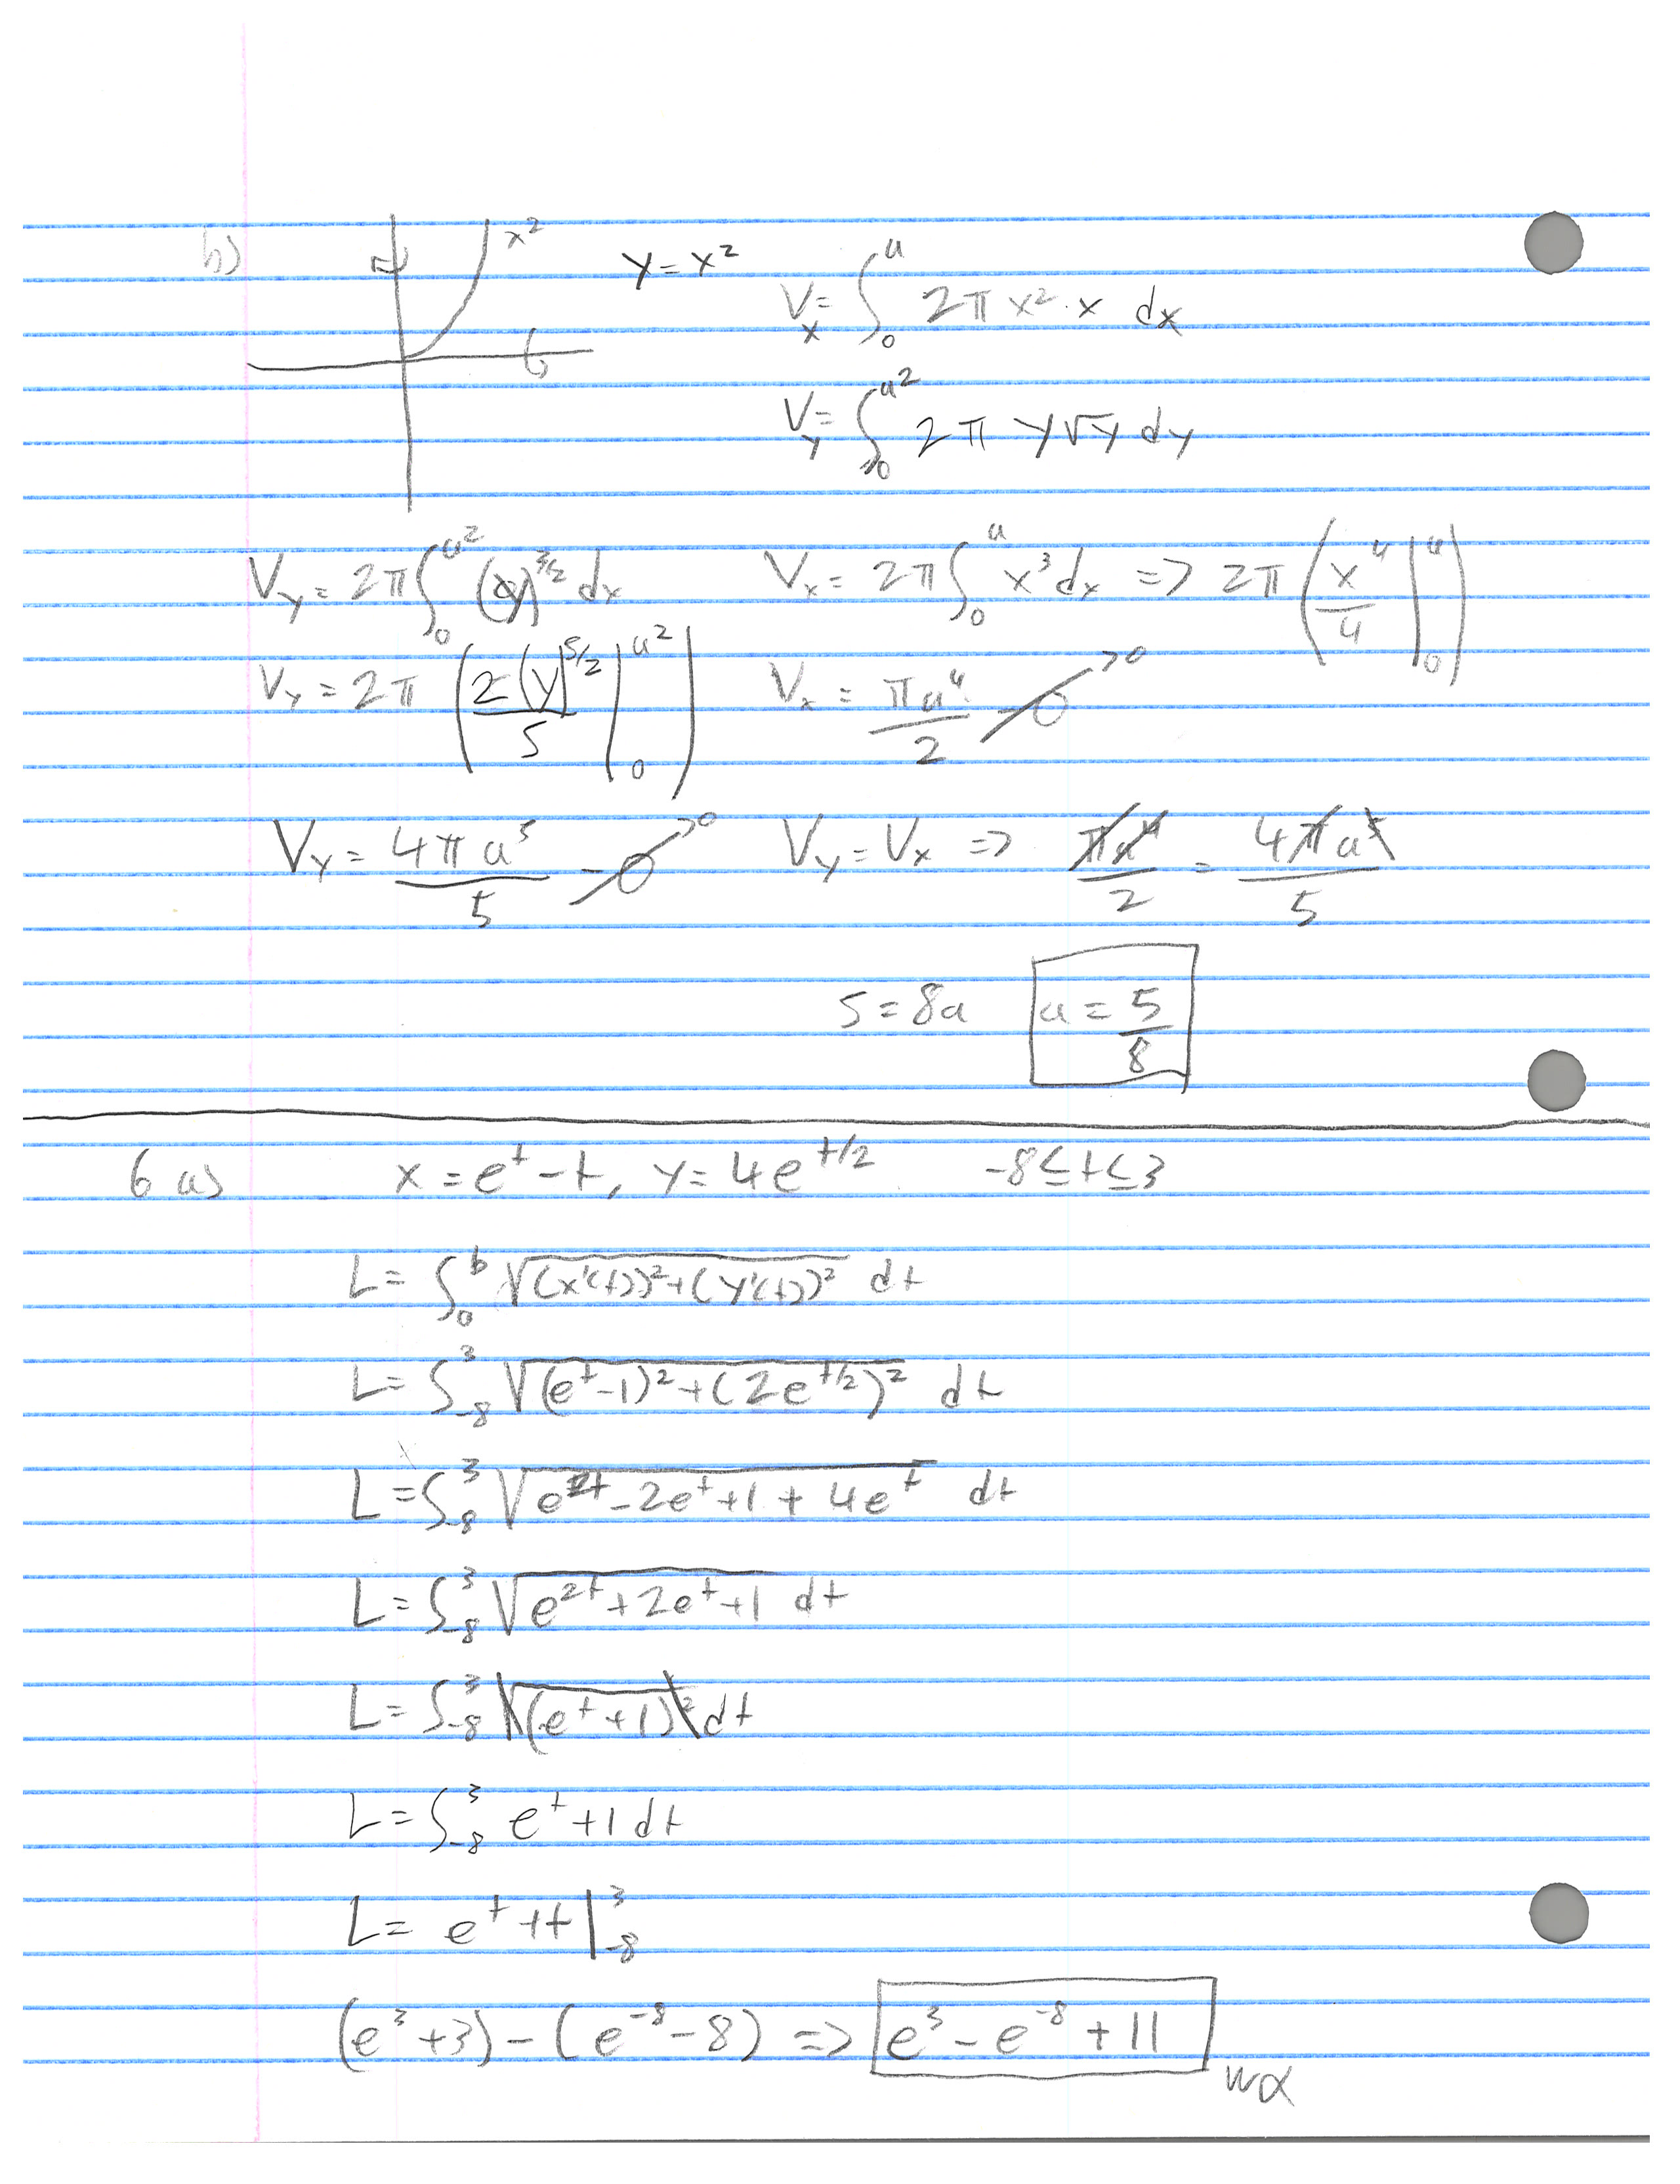
\includegraphics[trim={0 14cm 0 0},clip,scale=0.33]{./figures/math-final-work006.jpg}\\}
    \end{enumerate}
    
    \item Find the solution of the differential equation \((x^2 + 1)y' + 3xy = 3x\) that satisfies the condition $y(0) = 2$.
    \paragraph{Solution}
    \footnote{This is my vain attempt at in-lining Wolfram Alpha code into latex via automation, it was not pleasant.} 
    \begin{gather*}
        \frac{dy(x)}{dx} = \frac{3(-x + x y(x))}{x^2 + 1}\\
        \frac{dy(x)}{dx} = \frac{x(-3y(x)+3)}{x^2 + 1}\\
        \frac{ \frac{dy(x)}{dx}}{-3y(x) + 3} = \frac{x}{x^2 + 1}\\
        \int_{}^{} \frac{ \frac{dy(x)}{dx}}{-3y(x) + 3} = \int_{}^{} \frac{x}{x^2 + 1}\\
        - \frac{1}{3}\ln(-3y(x) + 3) = \frac{1}{2}\ln(x^2 + 1) + C\\
        y(x) = - \frac{C}{(x^2 + 1)^{3/2}} + 1\\
        \text{Solving for C}\\
        2 =  - \frac{C}{((0)^2 + 1)^{3/2}} + 1\\
        2 =  - \frac{C}{(1)^{3/2}} + 1\\
        - 1 = C\\
        y(x) = \frac{1}{(x^2 + 1)^{3/2}} + 1\\
    \end{gather*}
    \item Consider the following curve in parametric form: $ x = e^t - t,\ y = 4e^{t/2},\ -8 \leq t \leq 3$.
    \begin{enumerate}
        \item Determine the length of the curve
        \paragraph{Solution}~\\
        {\centering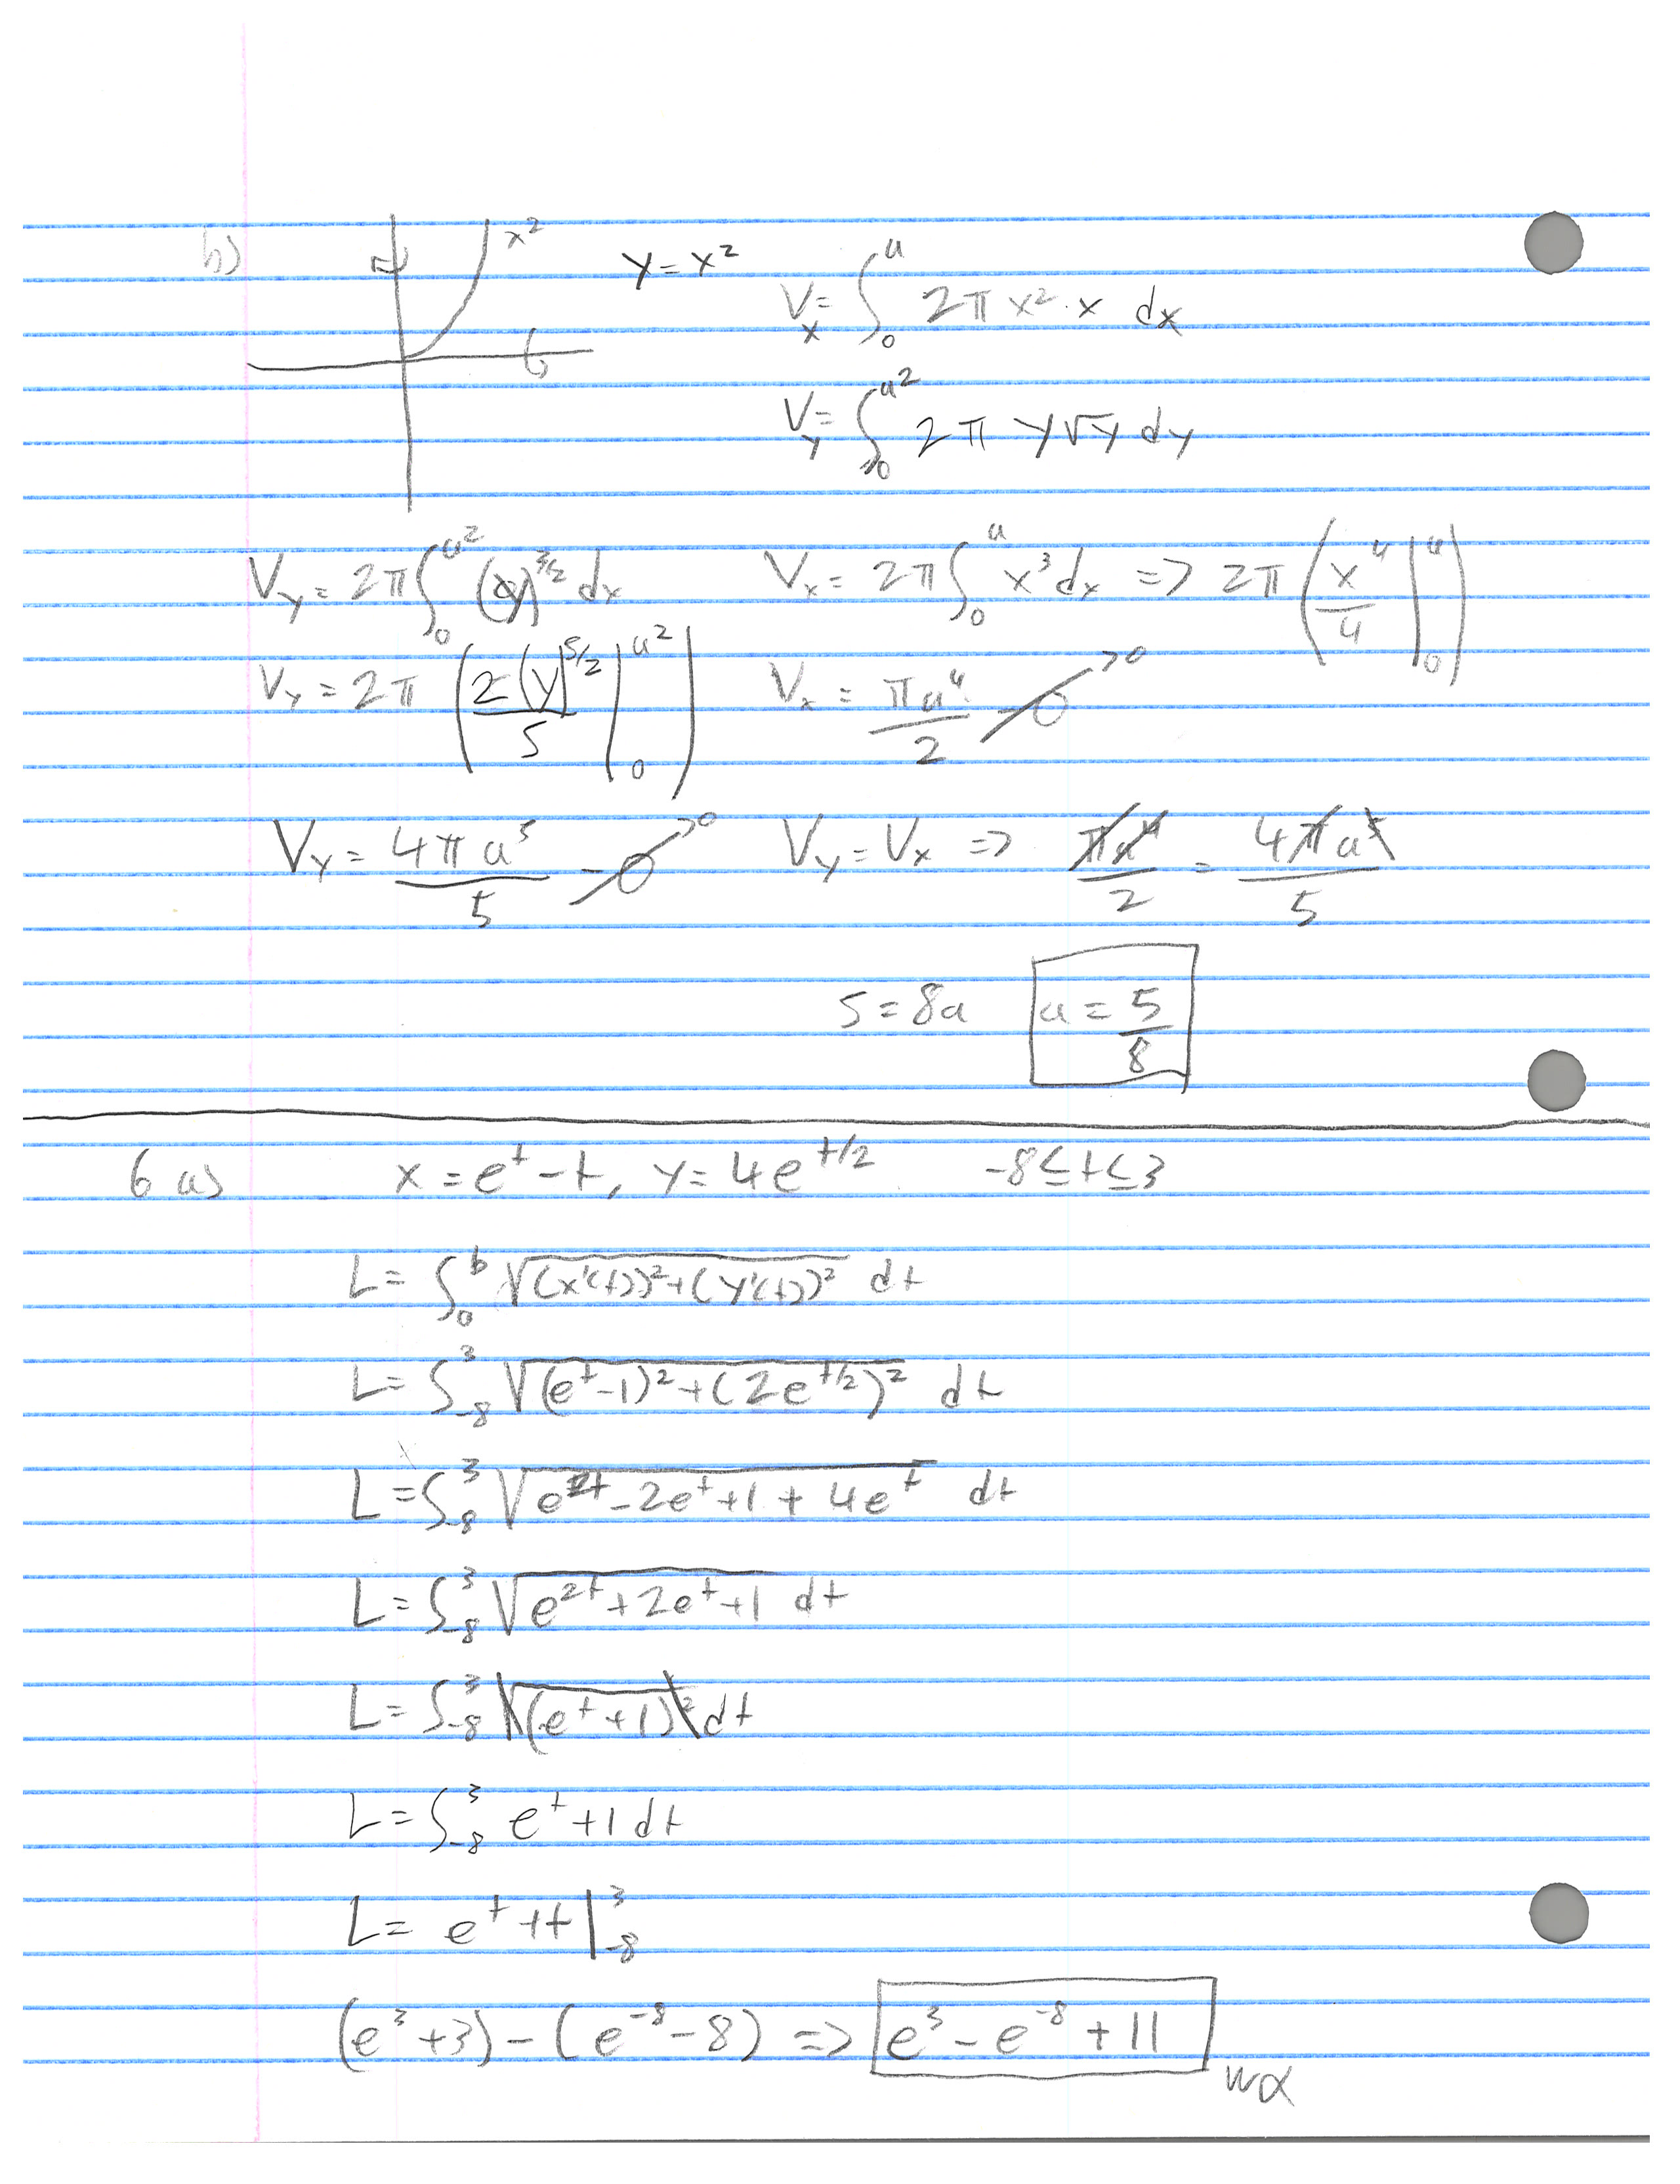
\includegraphics[trim={0 0 0 15cm},clip,scale=0.33]{./figures/math-final-work006.jpg}\\}
        \item Find the surface area obtained by rotating the curve about the x-axis.
        \paragraph{Solution}~\\
        {\centering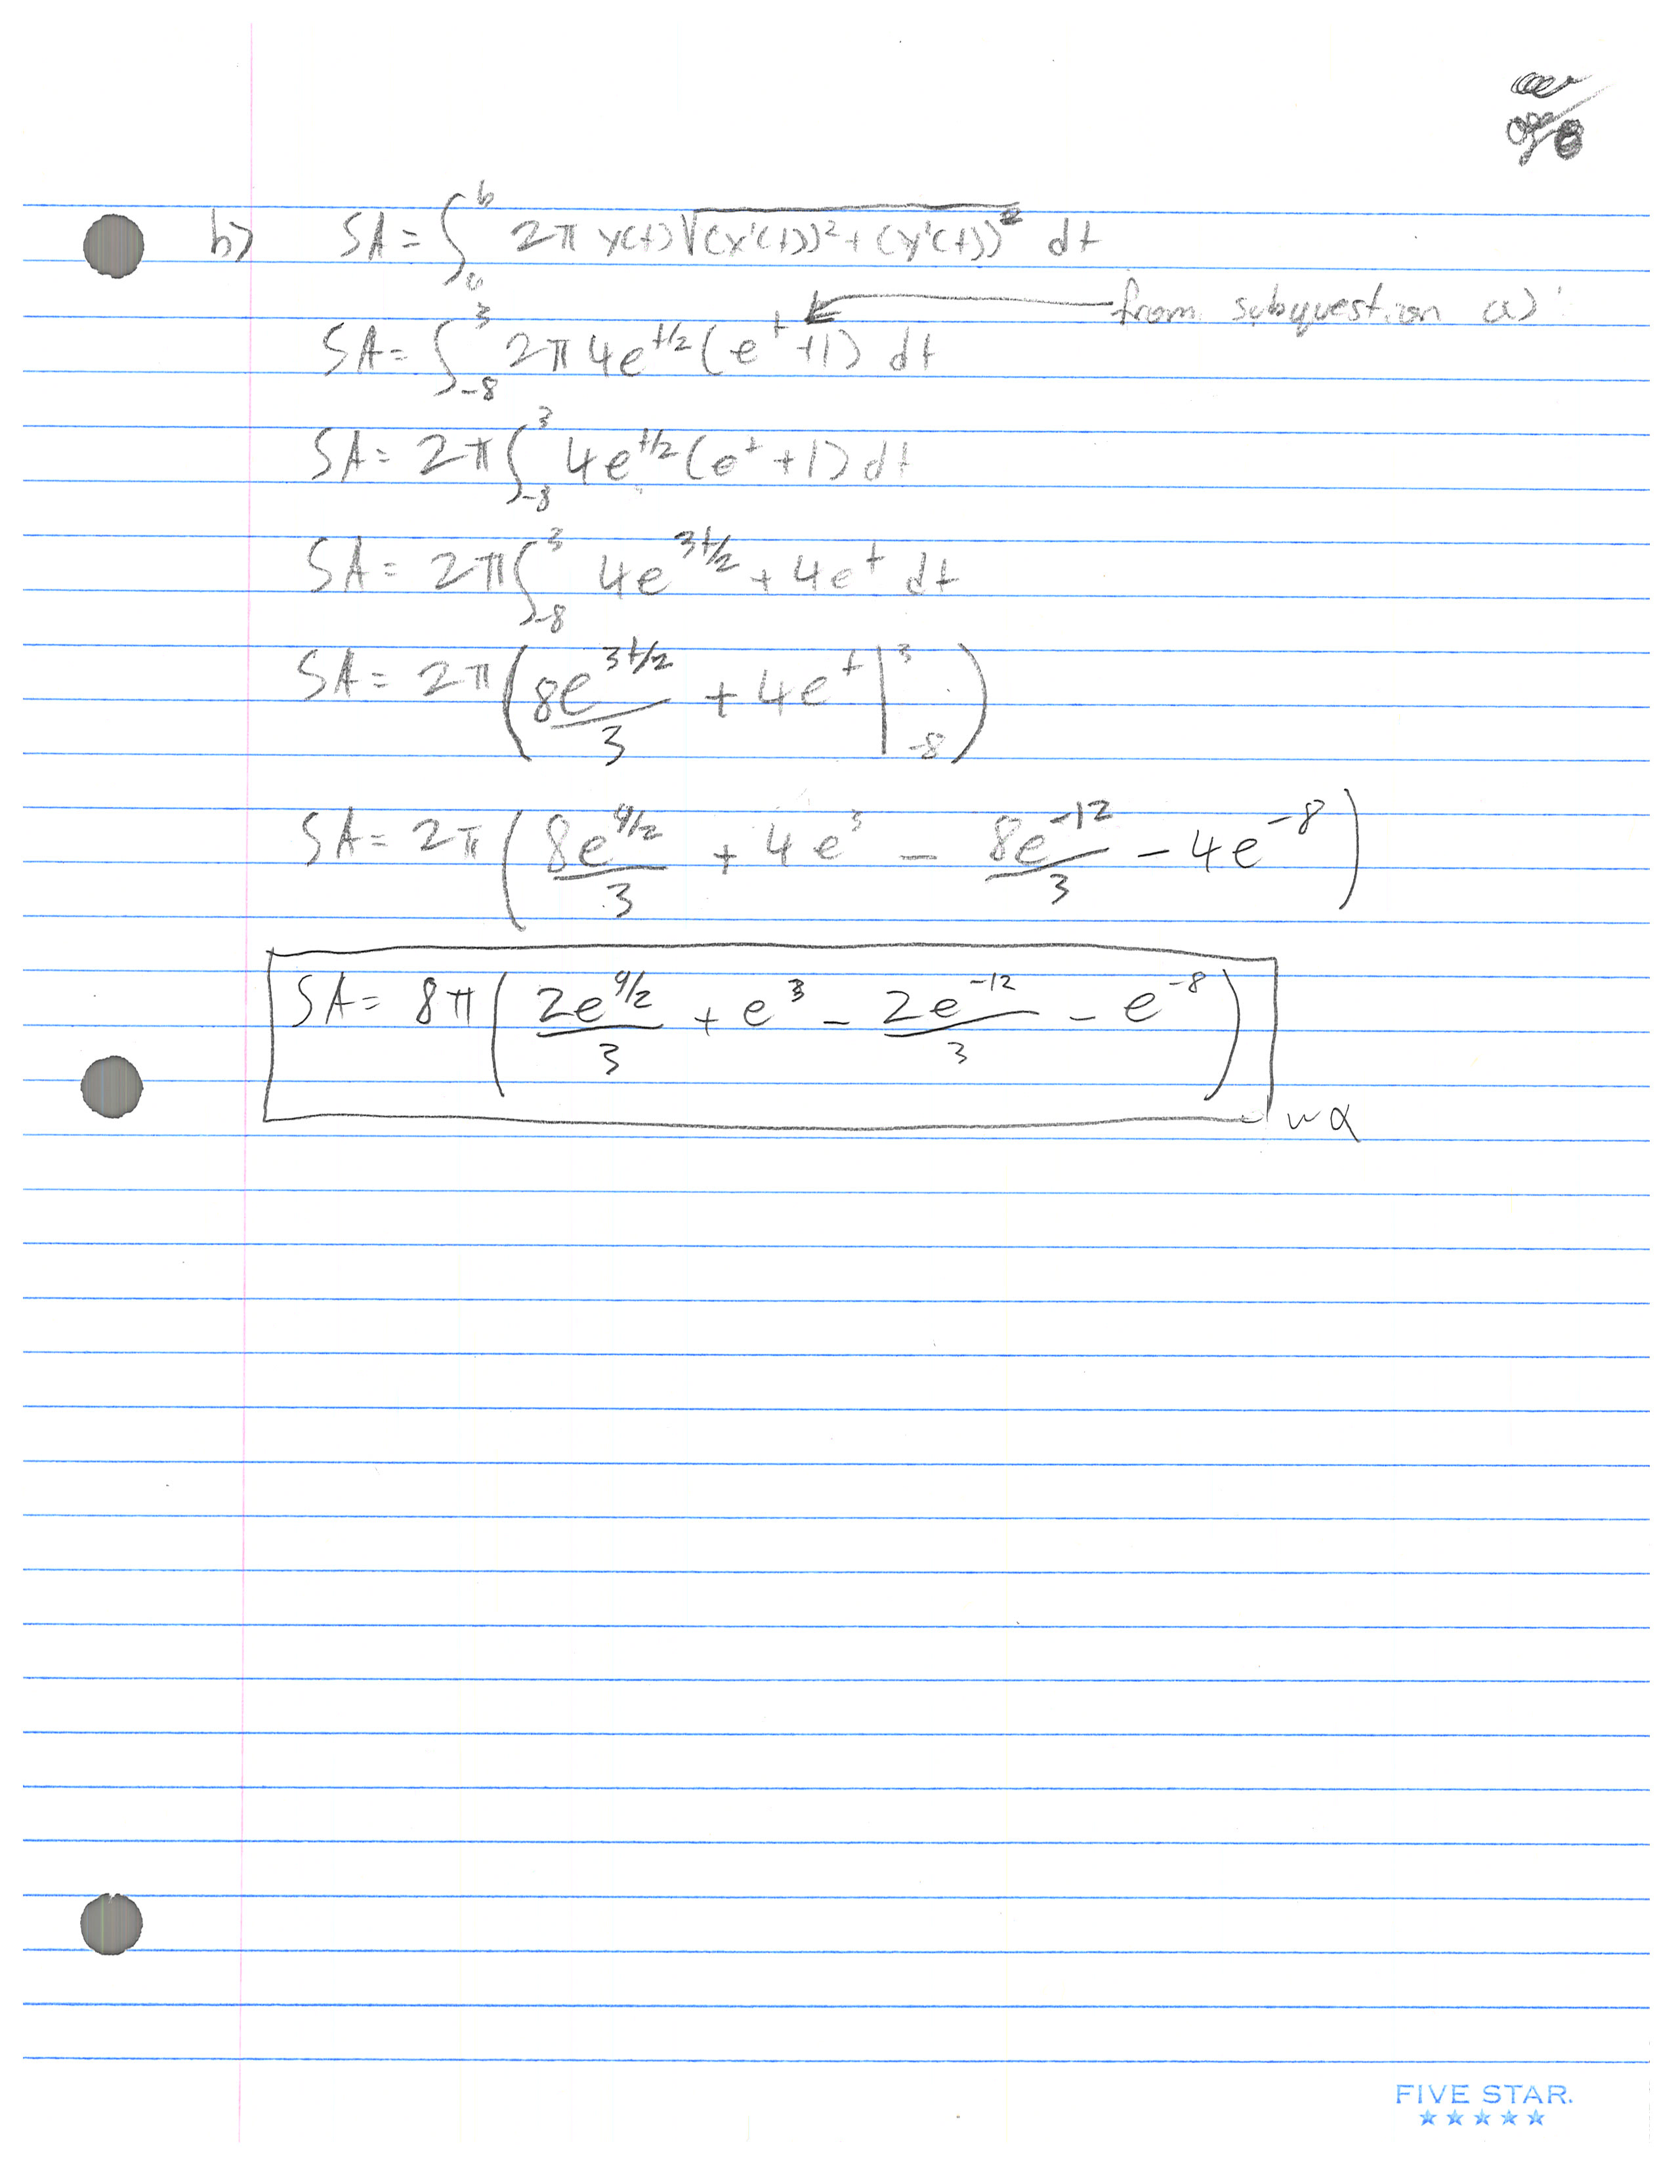
\includegraphics[trim={0 14cm 0 0},clip,scale=0.33]{./figures/math-final-work007.jpg}\\}
    \end{enumerate}
\end{enumerate}

\section{W18-MATH 115 R1 Final}
\begin{enumerate}
    \item Calculate \[\int_{0}^{\infty}\frac{\arctan x}{1+x^2}dx\]
    \paragraph*{Solution}
    \begin{gather*}
        \lim_{r \to \infty} \int_{0}^{r}\frac{\arctan x}{1+x^2}dx\\
        \text{Let } u = \arctan x\\
        \text{Then } du = \frac{dx}{1 + x^2}\\
        \lim_{r \to \infty} \int_{0}^{r} u\ du\\
        \lim_{r \to \infty} \frac{u^2}{2}\Big|_0^r\\
        \lim_{r \to \infty} \frac{\arctan^2(x)}{2}\Big|_0^r\\
        \lim_{r \to \infty} \frac{\arctan^2(r)}{2} - \frac{\arctan^2(0)}{2}\\
        \frac{\left( \frac{\pi}{4} \right)^2}{2} - \frac{0}{2}\\
        \frac{\pi^2}{8} - 0\\
        = \frac{\pi^2}{8}
    \end{gather*}
    \newpage


\end{enumerate}
\newpage
\section{F18-MATH 115 Final}
\subsection{Long Answer}
\begin{enumerate}
    \item Find the following integral \[\int_{0}^{1}xe^{3x}dx\]
    \paragraph*{Solution}
    We will use integrating by parts
    \begin{gather*}
        \text{Let: } u = x,\ du = dx,\ dv = e^{3x}dx,\ v = \frac{e^{3x}}{3}\\
        \frac{xe^{3x}}{3}\Big|_0^1 - \frac{1}{3} \int_{0}^{1} e^{3x}dx\\
        \frac{(1)e^{3(1)}}{3} - \cancelto{0}{\frac{(0)e^{3(0)}}{3}} = \frac{e^{3}}{3}\\
        \frac{1}{3} \int_{0}^{1} e^{3x}dx = \frac{1}{3} \left( \frac{e^{3x}}{3}\Big|_0^1 \right)\\
        \frac{1}{9}(e^3 - 1)\\
        \text{Combine with the first term}\\
        \frac{e^{3}}{3} - \frac{1}{9}(e^3 - 1)\\
        \frac{1}{9}(2e^3 + 1)
    \end{gather*}


    \item Find the following integral \[\int_{0}^{\pi/4}\tan^4(x)\sec^4(x)dx\]
    \paragraph*{Solution}
    \begin{gather*}
        \int_{0}^{\pi/4} \tan^4(x)(\sec^2(x))^2\ dx\\
        \int_{0}^{\pi/4} \tan^4(x) (1 + tan^2(x)) \sec^2(x)\ dx\\
        \text{Let } u = \tan(x),\ du = sec^2(x)\ dx\\
        \int_{0}^{1} u^4 (1 + u^2)\ du\\
        \int_{0}^{1} u^4 + u^6\ du\\
        \frac{u^5}{5} + \frac{u^7}{7}\Big|_0^1\\
        \left( \frac{1}{5} + \frac{1}{7}  \right) - 0\\
        = \frac{12}{35}
    \end{gather*}


    \item {If} \[\int_{0}^{1}f(x)dx = 2\] {\centering and \(f(2x) = 4f(x)\) find\\} \[\int_{1/2}^{1}f(x)dx\]
    \paragraph*{Solution}
    \begin{gather*}
        \text{The recurrence equation is } f(x) = \frac{Cx^2}{4}\\
        \int_{0}^{1} \frac{Cx^2}{4}dx = 2\\
        \frac{Cx^3}{12} \Big|_0^1 = 2\\
        \frac{C}{12} - 0 = 2\\
        C = 24\\ 
        \int_{1/2}^{1}6x^2dx\\
        2x^3 \Big|_{1/2}^1 = 2 - \frac{1}{4}\\
        = \frac{7}{4}
    \end{gather*}
    \begin{commentbox}{Note}
        I'm not too sure if this is the correct answer. Wolfram Alpha stated that this expression $f(2x) = 4f(x)$ is a recurrence equation of \[f(x) = \frac{Cx^2}{4}.\] Which kinda makes sense as you double the domain you quadruple the range, it looks like a quadratic relationship.
    \end{commentbox}
        



    \item Determine whether the following integral converges or diverges \[\int_{0}^{\infty}\frac{dx}{x^2+\sin^2(x)}\]
    \paragraph*{Solution}
    This function will always grows when the domain is greater than 0, so therefore we can set our lower bound to 0.\\
    \(x^2 + \sin^2(x)\) will grow faster than \(x,\ \forall x\in \mathbb{R},\ \text{where } x \geq 0\). Therefore.
    \begin{gather*}
        0 \leq \int_{0}^{\infty}\frac{dx}{x^2+\sin^2(x)} \leq \int_{0}^{\infty} \frac{dx}{x}\\
        \lim_{r \to \infty} \int_{0}^{r} \frac{dx}{x}\\
        \lim_{r \to \infty} \ln|x|\Big|_0^r\\
        \ln|r| - \ln|0|\\
        \infty - (-\infty)\\
        = \infty
    \end{gather*}
    Because the upper-bound is infinite the expression above is divergent. $\blacksquare$

    \newpage


    \item A pot of soup is placed into a refrigerator which is set at a temperature \(T_e = 5^{\circ}\). At $T = 75^{\circ}$, the temperature of the pot drops at a rate of -2c/s. Find the time when the temperature of the pot is $T = 30^{\circ}$ if we know $T_0 = 80^{\circ}$.
    \paragraph*{Solution} I solved this on page 20.


    \item A particle is moving in the xy plane according to the parametric function \(x(t) = t^2 + 2t\) and \(y(t) = t\) for \(-4 \leq t \leq 2\).
    \begin{enumerate}
        \item Find the velocity vector and the speed of the particle at $t=0$.
        \paragraph*{Solution}
        \begin{gather*}
            \vec{V}(t) =\ < x'(t),y'(t)>\\
            V(t) = \sqrt{(x'(t))^2 + (y'(t))^2}\\
            \vec{V}(t) =\ < 2t + 2, 1>\\
            V(t) = \sqrt{(2t + 2)^2 + 1^2}\\
            V(t) = \sqrt{4t^2 + 8t + 5}\\
            \vec{V}(0) =\ <2(0) + 2, 1>\ \Rightarrow\ <2,1>\\
            V(0) = \sqrt{4(0)^2 + 8(0) + 5}\\
            V(0) = \sqrt{5}
        \end{gather*}
        \item Determine the interval of $t$ when the path of the particle is concave down.
        \paragraph*{Solution} 
        \begin{gather*}
            \frac{d^2y}{dx^2} = \frac{y''(t)x'(t) - y'(t)x''(t)}{(x'(t))^3}\\
            = \frac{(0)(2t + 2) - (1)(2)}{2t + 2}\ dt\\
            = \frac{-2}{2t + 2}\ dt\\
            \text{The denominator will use of the number is going to be positive or negative}\\
            2t = -2 \Rightarrow t = -1\\
            \text{We want the denominator to be negative so } t < -1\\
            \text{So the interval will be } (-\infty, -1)
        \end{gather*}
    \end{enumerate}
\end{enumerate}
\newpage
\subsection{Multiple Choice}
    

\begin{enumerate}[itemsep=5mm]
        \item The area enclosed between the curves \(y = 3x\) and \(y = x^3\) is: 
        \begin{tasks}(4)
            \task \(\frac{3}{4}\)
            \task \(\frac{7}{4}\)
            \task \(\frac{9}{4}\)
            \task none of them
        \end{tasks}
        \paragraph*{Solution}
        \begin{gather*}
            \text{First we need to find our domain, set the two curves to equal each other } 3x = x^3\\
            x = \pm\sqrt{3}\\
            \text{This is an odd function so we can do this.}\\
            \int_{-\sqrt{3}}^{\sqrt{3}} = 2 \int_{0}^{\sqrt{3}} 3x - x^3 dx\\ 
            2 \left( \frac{3x^2}{2} - \frac{x^4}{4}\Big|_0^{\sqrt{3}} \right)\\
            2 \left( \frac{3(\sqrt{3})^2}{2} - \frac{(\sqrt{3})^4}{4} - 0 \right) = 2\left(\frac{9}{2} - \frac{9}{4}\right) = 2\left(\frac{9}{4}\right)\\
            = \frac{9}{2}\qquad \text{None of them, d}
        \end{gather*}

        \item Let $y(t)$ be the solution to the initial value problem 
        \[\begin{cases}
            y' + y = t\\
            y(0) = 0
        \end{cases}\]
        Then $y(1)$ is 
        \begin{tasks}(4)
            \task \(-1\)
            \task \(e^{-1}\)
            \task \(e\)
            \task none of them
        \end{tasks}
        \paragraph*{Solution}
        \begin{gather*}
            p(t) = 1,\ \ \mu(t)=e^{\int_{}^{}1\ dt}\\
            e^ty' + e^ty = te^t\\
            \int_{}^{}\left( ye^t \right)' = \int_{}^{}te^t dt\\
            ye^t = \int_{}^{}te^t dt\\
            \text{Let } u = t,\ du = dt,\ dv = e^t dt,\ v = e^t\\
            \int_{}^{}te^t dt = te^t - \int_{}^{}e^t dt\\
            y(t) = \frac{te^t - e^t + C}{e^t}\\
            \text{Finding C, set t = 0}\\
            0 = \frac{(0)e^{(0)} - e^{(0)} + C}{e^{(0)}}\\
            0 = \frac{-1}{1} + C\\
            C = 1\\
            y(t) = \frac{te^t - e^t + 1}{e^t}\\
            y(1) = \frac{(1)e^{(1)}}{e^{(1)}}\\
            y(1) = \frac{1}{e^1} = e^{-1}\\
            \text{The answer is b}
        \end{gather*}
        \item The surface area generated by the rotation of the curve $y = x^2,\ 0 \leq x \leq 1$ around the y-axis is:
        \begin{tasks}(4)
            \task $\frac{\pi}{8}(\sqrt{5} - 2)$
            \task $\frac{\pi}{24}(5\sqrt{5} - 2)$
            \task $\frac{\pi}{3}(5\sqrt{5} - 2)$
            \task none of them
        \end{tasks}
        \paragraph*{Solution}
        Solved this on page 17. Its none of them

        \item The value of the integral \[I = \int_{0}^{2}\frac{dx}{4 + x^2}^{3/2}\] is equal to
        \begin{tasks}(4)
            \task \(\frac{1}{4}\)
            \task \(\frac{\sqrt{2}}{8}\)
            \task \(\frac{1}{8}\)
            \task none of them
        \end{tasks}
        \paragraph*{Solution}
        \begin{gather*}
            x = 2\tan(\theta),\ dx = 2\sec^2(\theta)d\theta\\
            I  = \int_{0}^{2}\frac{2\sec^2(\theta)d\theta}{(4 + (2+\tan(\theta))^2)^{3/2}}\\
            I  = \int_{0}^{2}\frac{2\sec^2(\theta)d\theta}{(4 + 4 \sec^2(\theta))^{3/2}}\\
            I  = \int_{0}^{2}\frac{2\sec^2(\theta)d\theta}{4\sqrt{4}(1+\tan^2(\theta))^{3/2}}\\
            I = \frac{1}{4}\int_{0}^{2}\frac{\sec^2(\theta)d\theta}{(\sec^2(\theta))^{3/2}}\\
            = \frac{1}{4} \int_{0}^{2}\frac{\sec^2(\theta)d\theta}{\sec^3(\theta)}\\
            = \frac{1}{4} \int_{0}^{2} \cos(\theta)d\theta\\
            = \frac{1}{4} \left( \sin(\theta) \Big|_0^2 \right)\\
            = \frac{1}{4} \left( \frac{x}{\sqrt{4 + x^2}} \Big|_0^2 \right)\\
            = \frac{1}{4}\left( \frac{2}{\sqrt{8}} - 0 \right)\\
            = \frac{1}{4\sqrt{2}} = \frac{\sqrt{2}}{8}\qquad \text{The answer is b}
        \end{gather*}
        \item The volume generated by the rotation of the area enclosed by the curves $y = x$ and $ y = x^3$ around the y-axis.
        \begin{tasks}(4)
            \task\(\frac{\pi}{10}\)
            \task \(\frac{\pi}{5}\)
            \task \(\frac{\pi}{2}\)
            \task none of them
        \end{tasks}
        \paragraph*{Solution}~\\
        {\centering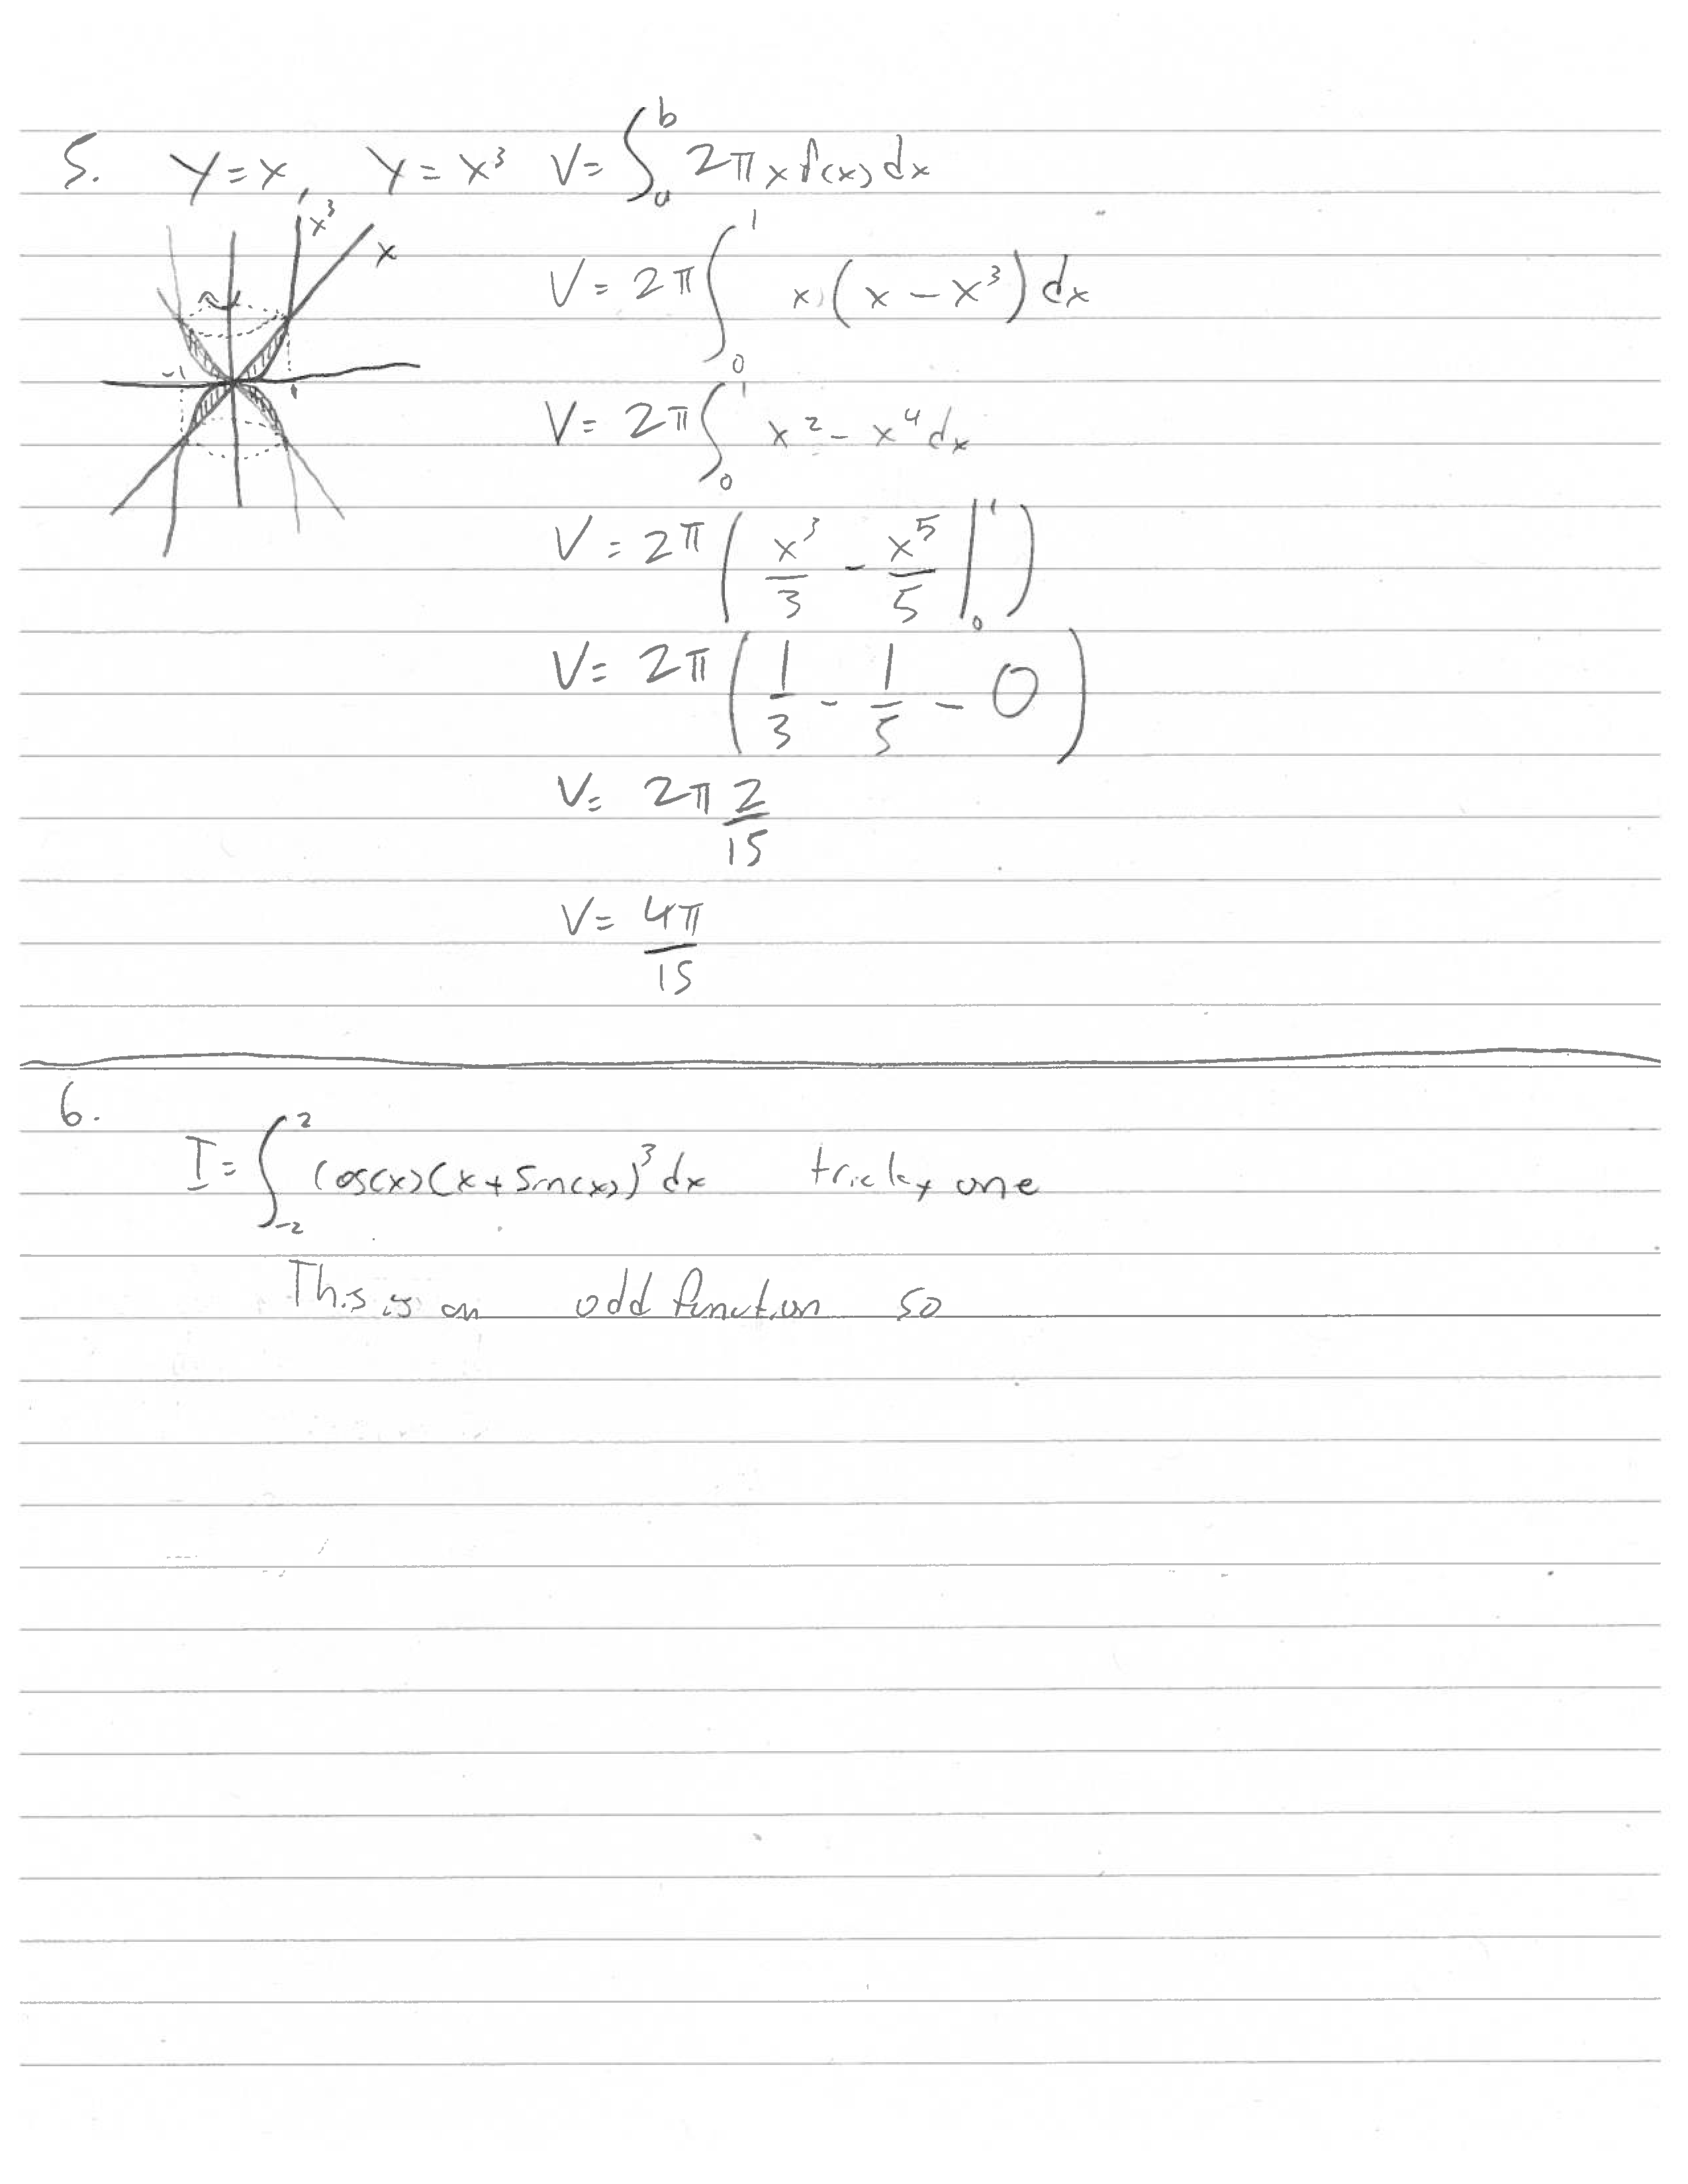
\includegraphics[trim={0 60cm 0 0},clip,scale=0.15]{./figures/output-0.png}\\}
        The answer is none of them.


        \item The value of the integral \[I = \int_{-2}^{2}\cos(x) (x + \sin(x))^3dx,\] is equal to
        \begin{tasks}(4)
            \task 1
            \task 0
            \task 2
            \task none of them
        \end{tasks}
        \paragraph*{Solution}
        This is a trick question question. Resist the urge to solve this, it will be a pain. This function $ \cos(x) (x + \sin(x))^3 $ is an odd function and the interval [-2,2] is symmetric about 0. Why?\\
        Well: cos is an even function $\cos(x) = \cos(-x)$, sin and x are odd functions $\sin(-x) = -\sin(x)$. For both functions their magnitude from the origin is the same. Since $x + \sin(x)$ is an odd function their magnitude or distance from the origin will be the same the only difference is the direction. Cubing them into $ (x + \sin(x))^3 $ also makes it an odd function. Multiplying this function with another even function will have the entire expression still be odd. Therefore so long as the domain is symmetric which means the entire function will have an area of zero as each side of the symmetric function cancel each other out. 
        \\~\\
        The answer is 0 or b.\\  
        
        {\centering \begin{tikzpicture}
            \begin{axis}[xmin=-2.5,ymin=-20,xmax=2.5,ymax=20, samples=300, axis lines = middle,xlabel=$x$,ylabel=$y$]
                \addplot[color=red]{ cos(deg(x))*((x + sin(deg(x)))^3)};
            \end{axis}
        \end{tikzpicture}\\}   
        \item The integral \[I = \int_{0}^{2}|x - 1|dx\]
        \begin{tasks}(4)
            \task 0
            \task 1
            \task 2
            \task none of them    
        \end{tasks}
        {\centering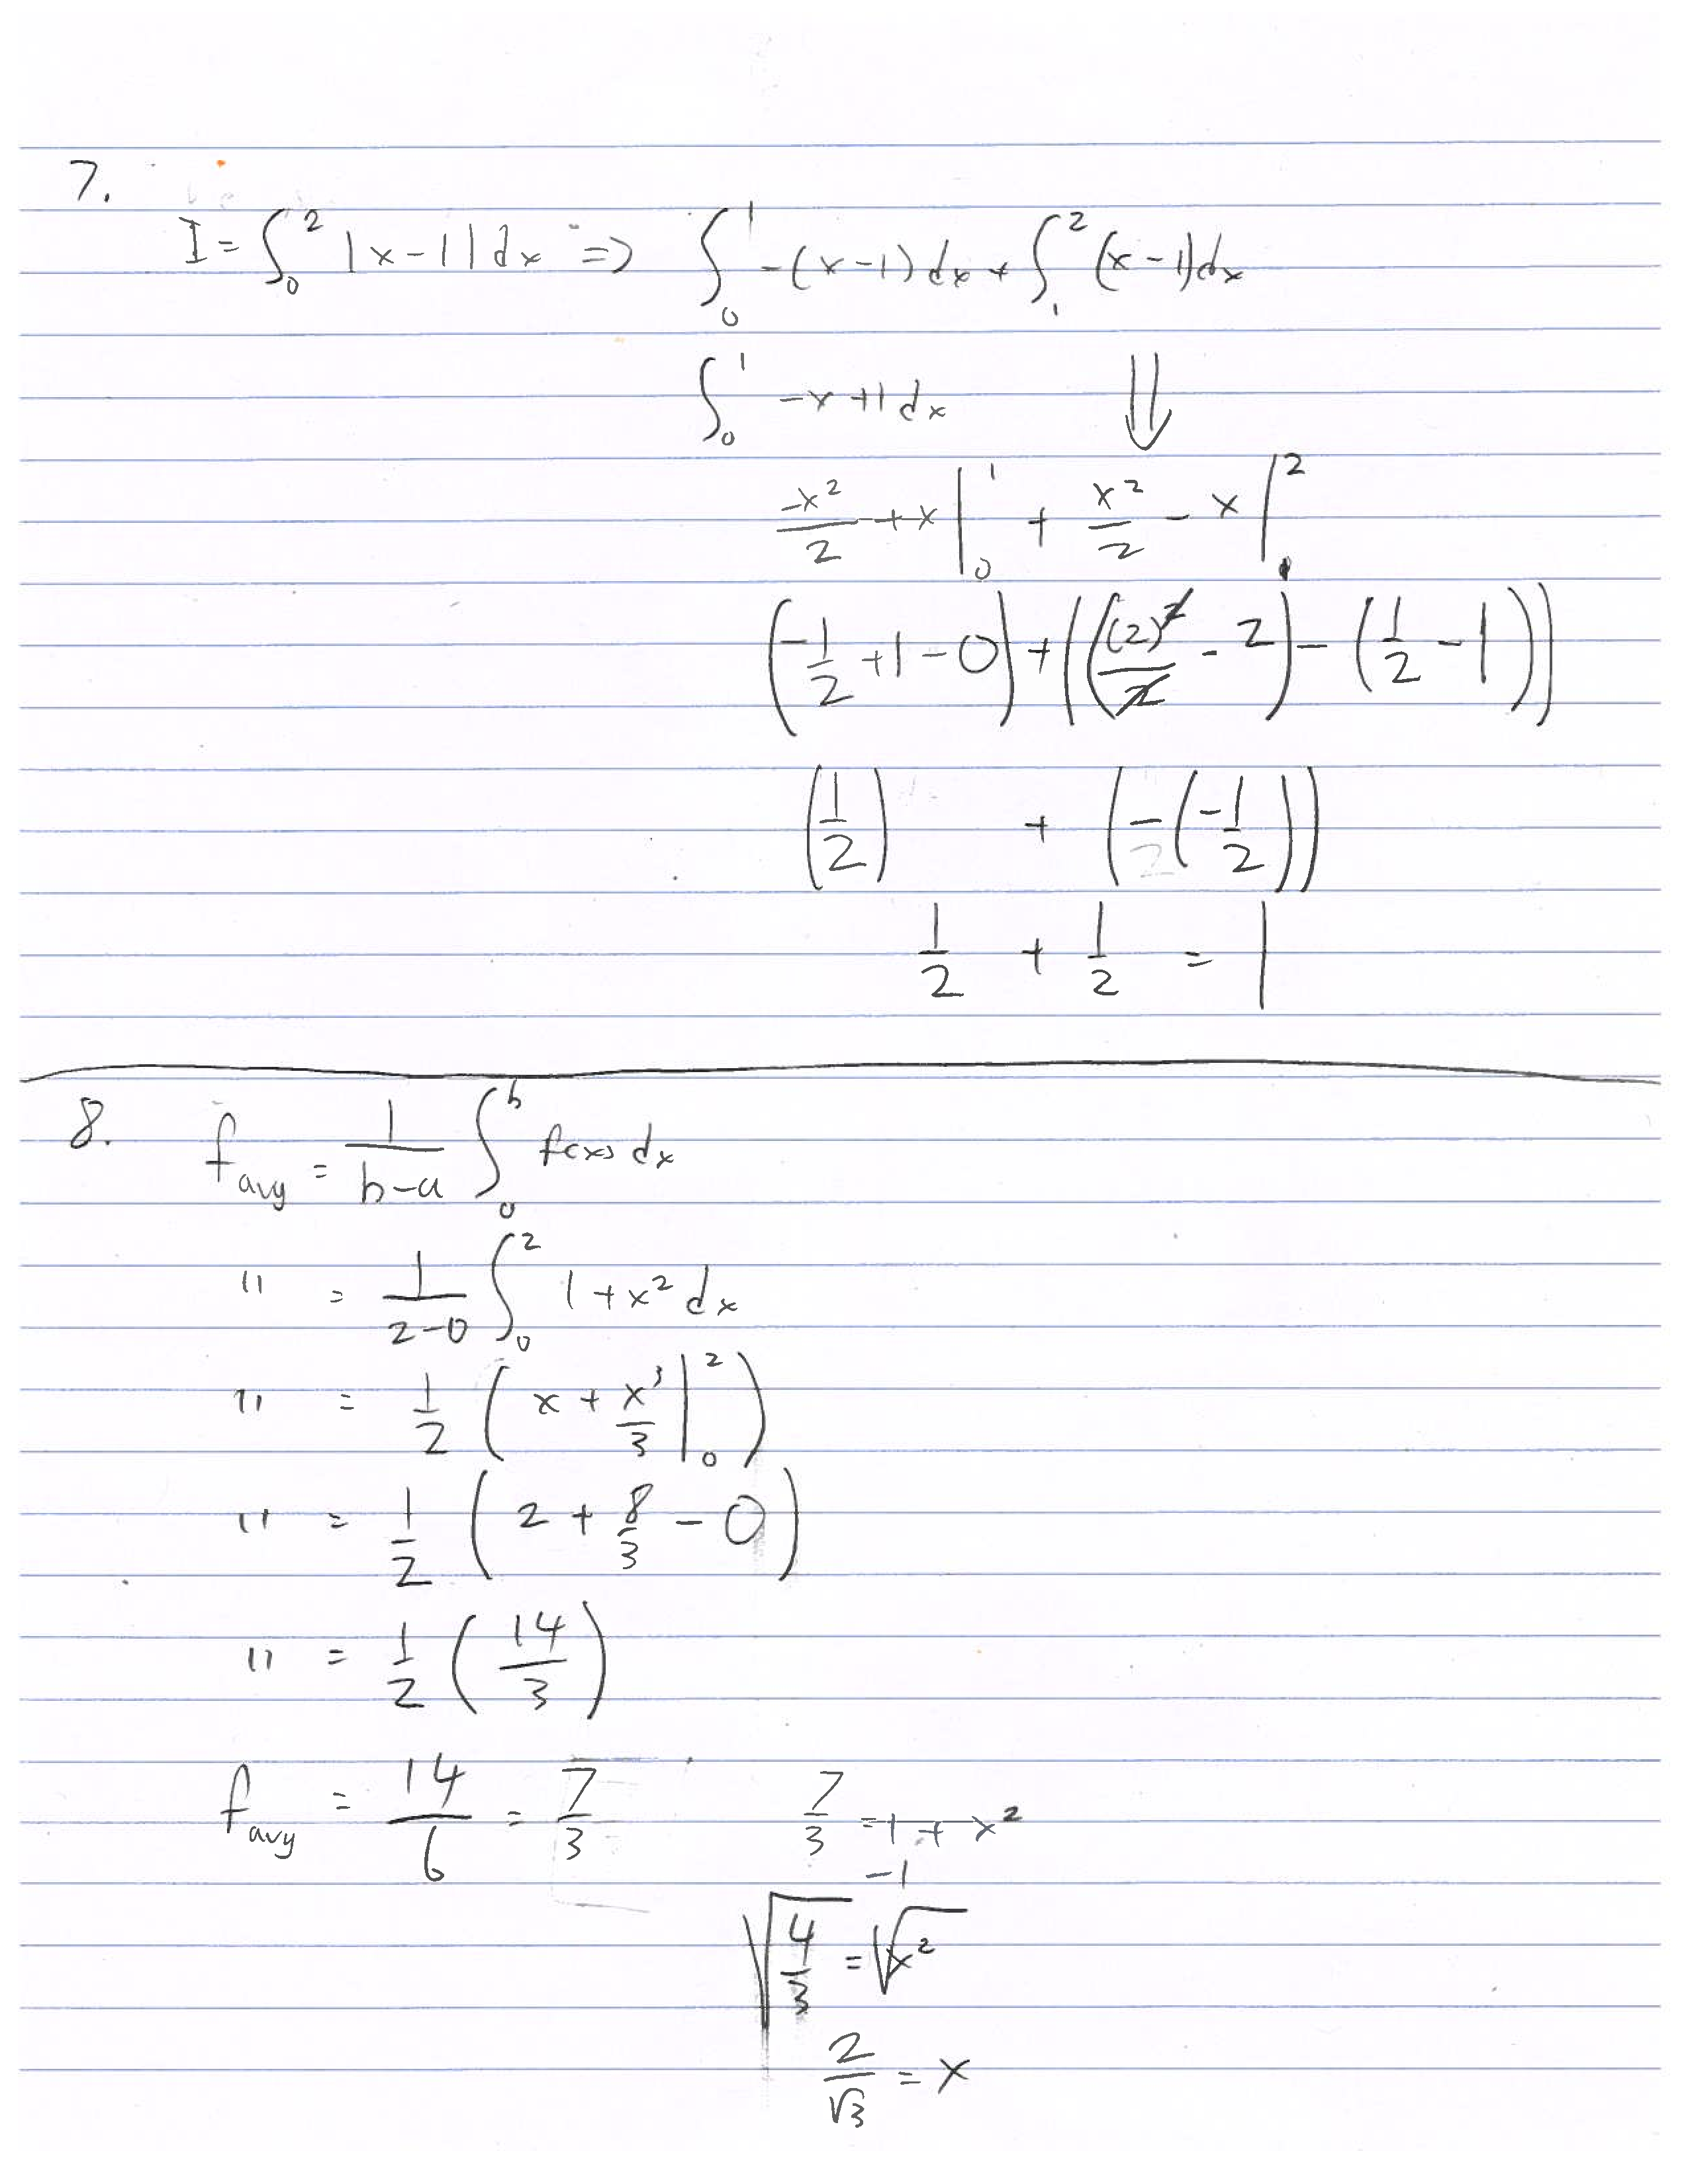
\includegraphics[trim={0 60cm 0 0},clip,scale=0.15]{./figures/output-1.png}\\}
        The answer is 1 or b.
        \item Consider the function $f(x) = 1 + x^2$ in [0,2]. Find $c\in[0,2]$ such that $f(c) = \bar{f}$, where $\bar{f}$ is the average of $f$ in the given interval.
        \begin{tasks}(4)
            \task \(\frac{2}{3}\)
            \task \(\frac{4}{\sqrt{3}}\)
            \task \(\frac{2}{\sqrt{3}}\)
            \task none of them
        \end{tasks}
        {\centering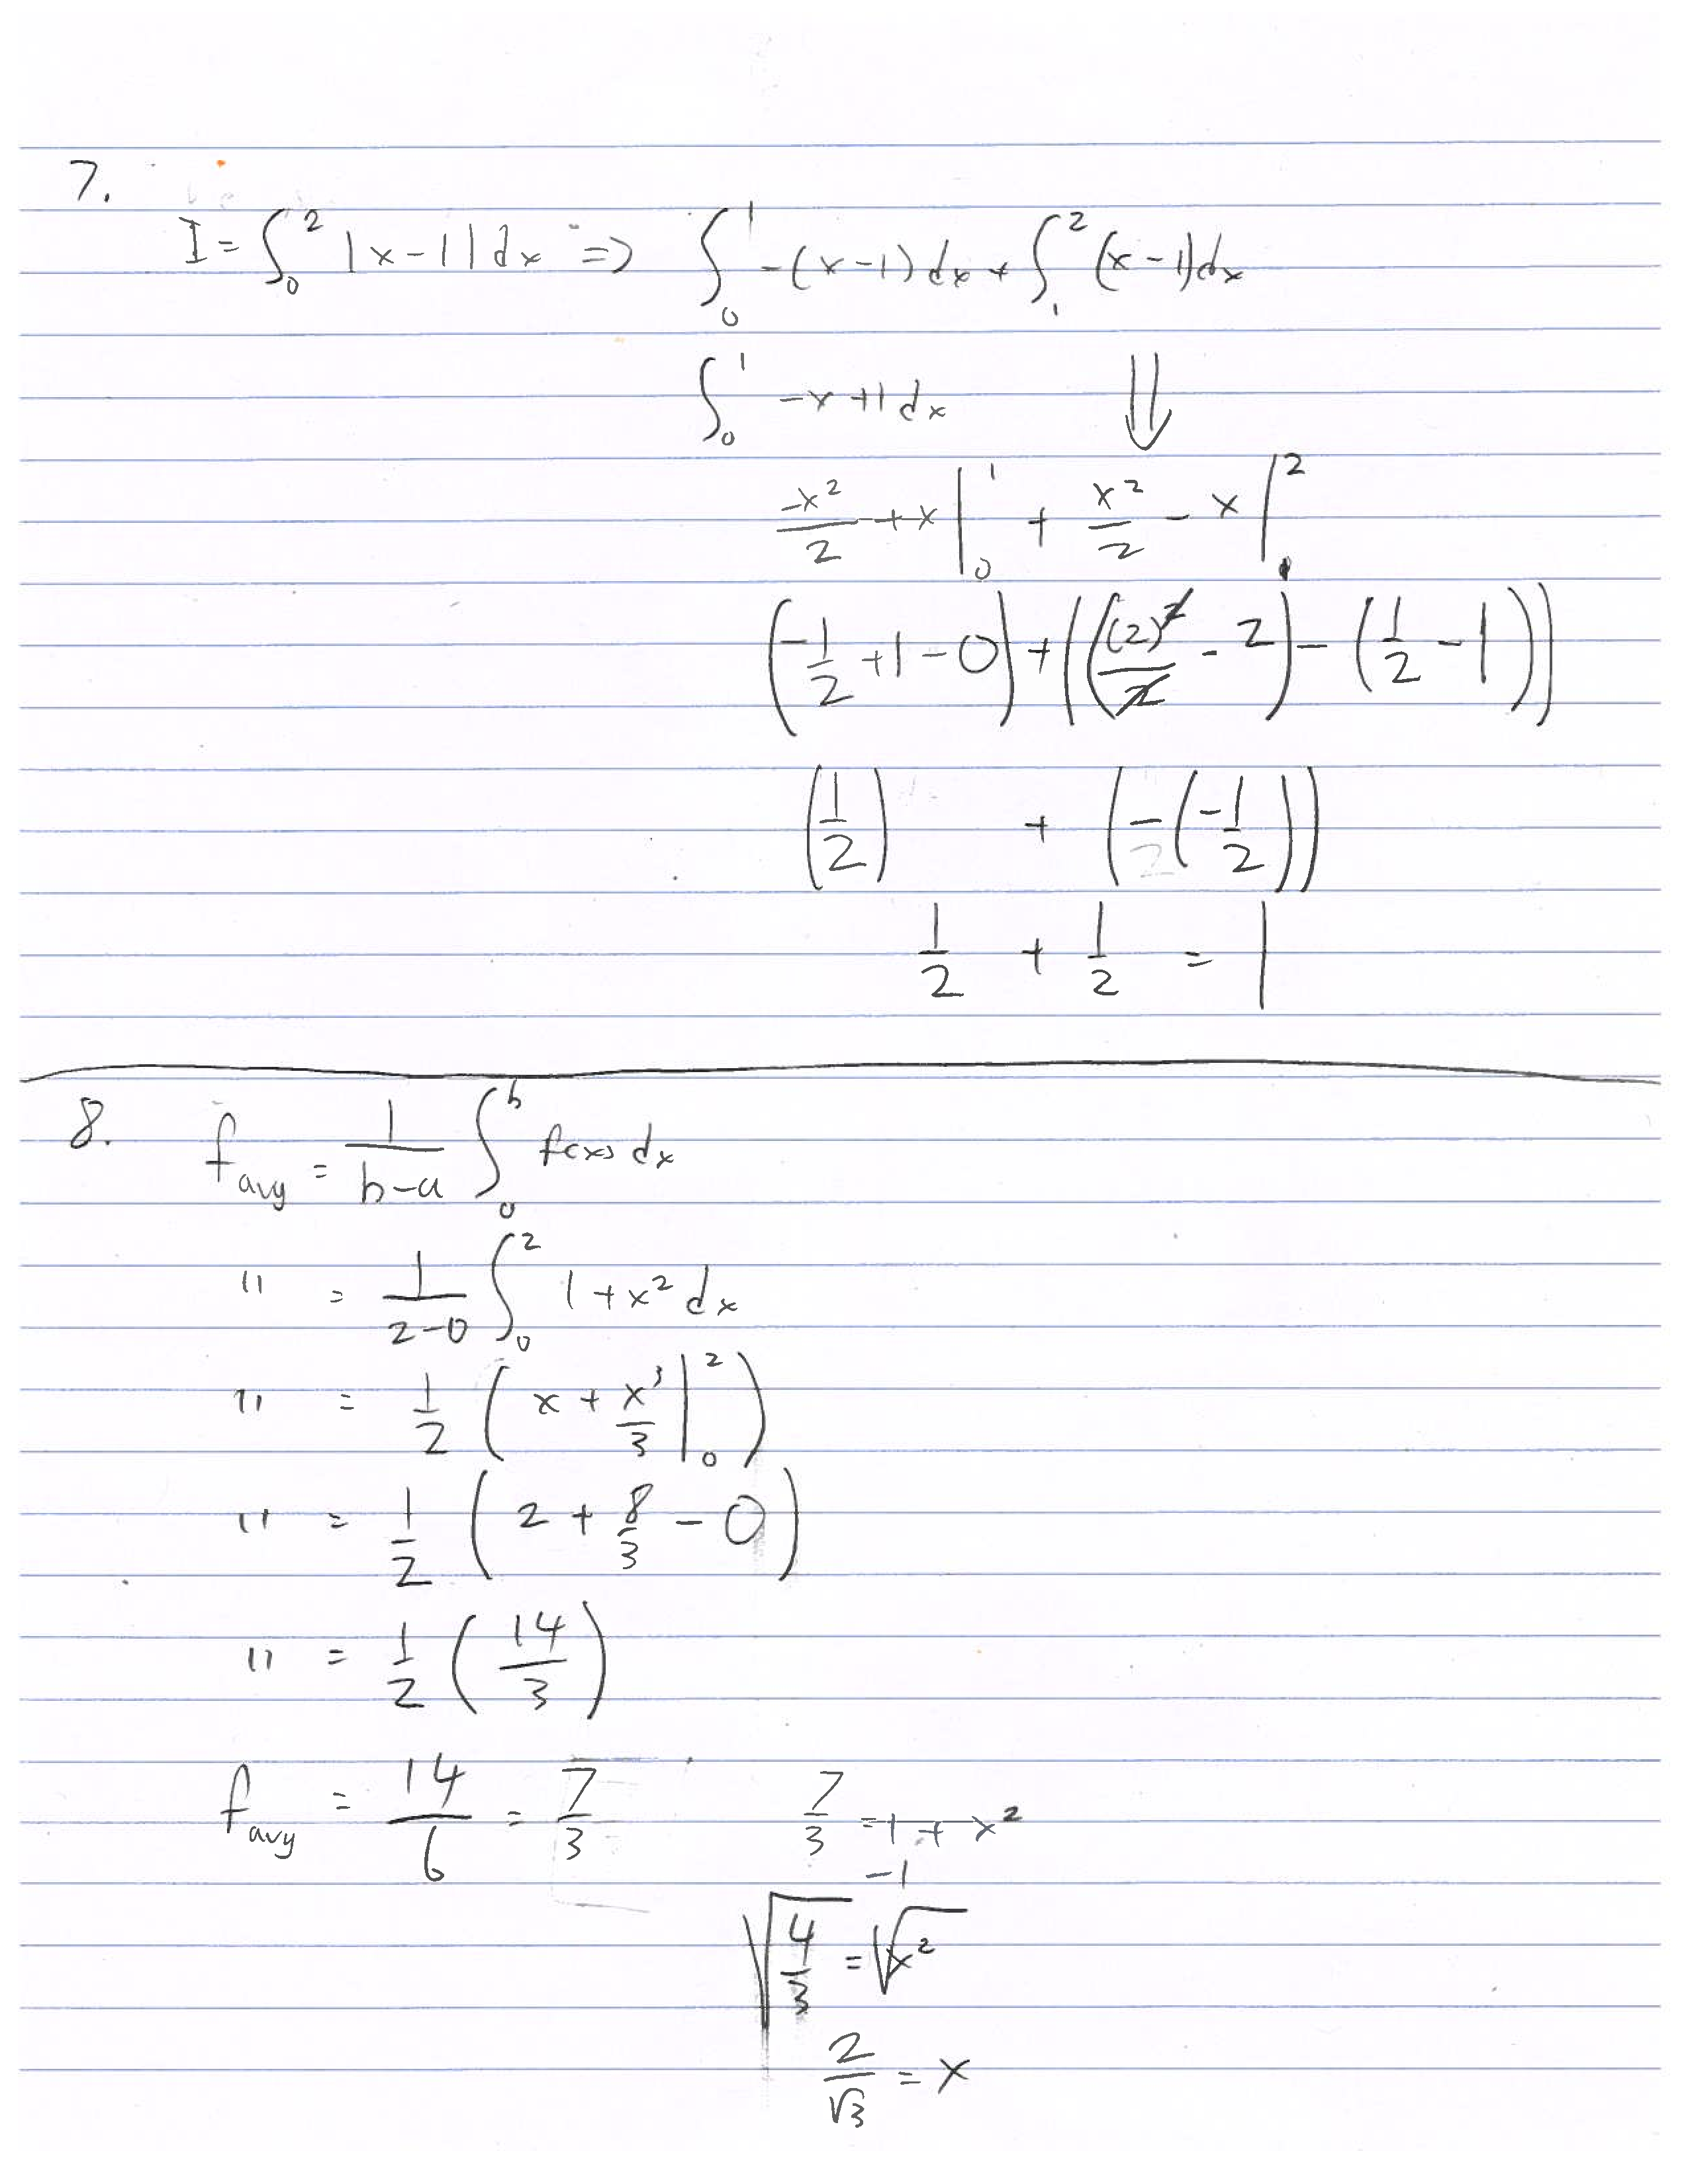
\includegraphics[trim={0 0 0 55cm},clip,scale=0.15]{./figures/output-1.png}\\}
        The answer is $\frac{2}{\sqrt{3}}$ or c.
\end{enumerate}
\end{document}